\documentclass[11pt]{article}
\usepackage[T1]{fontenc}
\usepackage[utf8]{inputenc}
\usepackage{lmodern}
\usepackage[margin=1in]{geometry}
\usepackage{amsmath,amssymb,amsthm,mathtools}
\usepackage{booktabs,array}
\usepackage{tikz-cd}
\usetikzlibrary{arrows.meta,positioning}
\usepackage[numbers,sort&compress]{natbib}
\usepackage{microtype}
\usepackage{xurl}
\usepackage{xcolor}
\usepackage[colorlinks=true,linkcolor=blue!45!black,citecolor=blue!45!black,urlcolor=blue!45!black]{hyperref}
\usepackage[capitalise,nameinlink,noabbrev]{cleveref}
\hypersetup{pdftitle={A counterexample to Tachikawa's second conjecture},pdfauthor={OpenAI}}
\DeclareMathOperator{\Hom}{Hom}
\DeclareMathOperator{\End}{End}
\DeclareMathOperator{\Ext}{Ext}
\DeclareMathOperator{\Tor}{Tor}
\DeclareMathOperator{\im}{im}
\DeclareMathOperator{\coker}{coker}
\DeclareMathOperator{\rad}{rad}
\DeclareMathOperator{\soc}{soc}
\DeclareMathOperator{\add}{add}
\DeclareMathOperator{\pd}{pd}
\DeclareMathOperator{\idim}{id}
\DeclareMathOperator{\domdim}{domdim}
\DeclareMathOperator{\tr}{tr}
\DeclareMathOperator{\Res}{Res}
\DeclareMathOperator{\Cone}{Cone}
\newcommand{\sHom}{\underline{\Hom}}
\newcommand{\sEnd}{\underline{\End}}
\newcommand{\cH}{\mathcal H}
\newcommand{\cI}{\mathcal I}
\newtheorem{theorem}{Theorem}[section]
\newtheorem{proposition}[theorem]{Proposition}
\newtheorem{lemma}[theorem]{Lemma}
\newtheorem{corollary}[theorem]{Corollary}
\theoremstyle{definition}
\newtheorem{definition}[theorem]{Definition}
\newtheorem{notation}[theorem]{Notation}
\theoremstyle{remark}
\newtheorem{remark}[theorem]{Remark}
\newtheorem{example}[theorem]{Example}
\numberwithin{equation}{section}
\setlength{\emergencystretch}{1.5em}
\title{A counterexample to Tachikawa's second conjecture}
\author{OpenAI}
\date{September 23, 2026}
\begin{document}
\maketitle
\begin{abstract}
We disprove Tachikawa's second conjecture by constructing a
finite-dimensional symmetric algebra over $k=\mathbb F_2(q,H_1,H_2)$
with a finite-dimensional nonprojective module whose self-extension
groups vanish in every positive degree. The associated endomorphism
algebra also gives
counterexamples to the classical, generalized, and strong Nakayama
conjectures, the Auslander--Gorenstein conjecture, and the Wakamatsu
tilting conjecture. These conclusions persist after every extension of $k$.
\end{abstract}
\section{Introduction}\label{sec:introduction}

Let $A$ be a finite-dimensional algebra over a field $k$.
A finite-dimensional $A$-module $M$ is \emph{self-orthogonal} if
$\Ext_A^i(M,M)=0$ for every integer $i>0$.
Tachikawa's second conjecture asserts that every finite-dimensional
self-orthogonal module over a finite-dimensional self-injective
algebra is projective.  This question belongs to the homological
conjectures surrounding quasi-Frobenius algebras and dominant
dimension; see Tachikawa's 1973 monograph~\cite[pp.~VI--VII]{Tachikawa1973} and the account
of the conjecture in~\cite[p.~7288]{ChenXi2025TAMS}.
The Auslander--Reiten conjecture, originating in
\cite{AuslanderReiten1975}, asks for finite-dimensional algebras
whether the condition $\Ext_A^i(M,M\oplus A)=0$ for every $i>0$
forces $M$ to be projective. For a self-injective algebra, the groups
$\Ext_A^i(M,A)$ vanish automatically, so Tachikawa's second conjecture
is its self-injective case.

Write $D=\Hom_k(-,k)$. An algebra $A$ is \emph{symmetric} if
$A\simeq DA$ as $A$-bimodules; in particular, a symmetric algebra
is self-injective. We prove the following result in this class.

\begin{theorem}\label{thm:main}
Let
\[
 k=\mathbb F_2(q,H_1,H_2),
\]
where $q,H_1,H_2$ are algebraically independent.
There exist a finite-dimensional associative unital symmetric
$k$-algebra $A$ and a finite-dimensional unital left $A$-module $M$
such that $M$ is nonprojective and
\[
 \Ext_A^i(M,M)=0\qquad\text{for every integer }i>0.
\]
In particular, Tachikawa's second conjecture is false.
\end{theorem}

Since $A$ is self-injective, the same module satisfies
$\Ext_A^i(M,M\oplus A)=0$ for every $i>0$.
Thus Theorem~\ref{thm:main} also gives a symmetric counterexample to
the Auslander--Reiten conjecture.

\paragraph{Related results.}
Schulz's earlier example of a nonprojective module without positive
self-extensions uses an algebra over a skew field, outside the
finite-dimensional-over-a-field setting considered here; see
\cite{Schulz1994} and the distinction recalled in
\cite[Introduction]{DiverisPurin2012}.
His quantum-exterior example has nonzero first self-extension but no
higher self-extensions
\cite[Example~7]{Schulz1995}; the parameter-shifting syzygies in that
example are an antecedent for our starting algebra.
For symmetric Artin algebras, Diveris and Purin show that a component
containing a nonprojective module with eventually vanishing
self-extensions has stable part of type $\mathbb Z A_\infty$
\cite[Theorem~A]{DiverisPurin2014}.
Over an algebraically closed field, Erdmann classifies, up to Morita
equivalence, the indecomposable
weakly symmetric algebras with radical cube zero and nonzero radical
square that admit such modules. The classification singles out quantum
exterior and double Nakayama algebras with parameters that are not roots
of unity~\cite[Theorem~1.1]{Erdmann2017}.

Chen, Fang and Xi characterize the symmetric case through stratifying
ideals and give conditional mirror-reflective constructions from
gendo-symmetric counterexamples to the Nakayama conjecture
\cite[Theorems~1.1 and~1.2]{ChenFangXi2024}.
Chen and Xi relate self-orthogonal Nakayama-stable generators over
self-injective algebras to additional categorical and
Gorenstein--Morita conditions~\cite[Theorem~1.2 and Corollary~1.4]{ChenXi2025TAMS}.
Their further criterion assumes virtual Gorensteinness of the relevant
endomorphism algebra~\cite[Theorem~1.3]{ChenXi2025VG}.
Zhang and Zhou prove the self-injective case for split algebras with
radical cube zero~\cite[Corollary~4.2]{ZhangZhou2026} and subsequently
treat Igusa--Todorov algebras~\cite[Theorem~3.2]{ZhangZhouIgusaTodorov2026}.
Xia proves the Auslander--Reiten conjecture for quantum complete
intersections~\cite[Corollary~4.3]{Xia2026}.
In a different direction, B\"ohmler and Marczinzik construct a
nonprojective module over a commutative local self-injective algebra
whose first two self-extension groups vanish, while the third does
not~\cite[Theorem~3.1 and the end of Section~3]{BohmlerMarczinzik2026}.
Theorem~\ref{thm:main} establishes vanishing in every positive degree.

Enomoto and Marczinzik prove that Tachikawa's second conjecture for the
two-fold trivial extension of an Artin algebra implies the Auslander--Reiten
conjecture for that algebra~\cite[Theorem~3.5]{Enomoto2026}.
This reduction has a self-injective target, not a symmetric target in
general. Our construction obtains a symmetric algebra by establishing
the additional complete-resolution vanishing needed for transfer to
the ordinary trivial extension.
Enomoto and Marczinzik also prove an equivalence among the universal
versions of the Auslander--Reiten, generalized Nakayama, Nakayama,
and both Tachikawa conjectures
over a fixed commutative Artinian coefficient
ring~\cite[Theorem~1.1]{Enomoto2026}.

\paragraph{The construction.}
The companion article~\cite{OpenAIAR2026} constructs an explicit
eight-simple triangular counterexample. We use the same ten-dimensional
starting algebra and related cone and triangular-module constructions,
and reproduce the algebra, resolutions, and arguments needed here.
The passage to a symmetric algebra requires vanishing in negative
degrees of a complete self-extension complex as well as positive Ext
vanishing.

Two steps organize the proof.  First, Proposition~\ref{tr:transfer}
gives a general transfer principle. For a finite-dimensional algebra
$\Lambda$, a doubly infinite exact complex $P_Z$ of finite projective
$\Lambda$-modules is \emph{totally acyclic}
if $\Hom_\Lambda(P_Z,\Lambda)$ is also exact. Suppose
$P_Z$ is totally acyclic, $Z=\coker((P_Z)_1\to(P_Z)_0)$, and
\begin{equation}\label{intro:profile}
 H^a\Hom_\Lambda(P_Z,Z)=0
 \qquad(a>0\ \text{or}\ a\leq-2).
\end{equation}
Then the trivial extension and induced module
\[
 A=\Lambda\ltimes D\Lambda,
 \qquad M=A\otimes_\Lambda Z
\]
give the required symmetric example whenever $Z$ is nonprojective.
The negative tail computes the positive extensions into
$D\Lambda\otimes_\Lambda Z$, with the precise index $-a-1$.
This transfer principle applies to any finite-dimensional algebra
and module satisfying its hypotheses.

Second, we construct the data required by this transfer. A
ten-dimensional algebra $C$ has a one-dimensional simple module $s$.
Put
\[
 T=C\ltimes DC,\qquad B=C\otimes_k C,
 \qquad E=T\otimes_k T,\qquad X=s\otimes_k s.
\]
We regard $s$ as a $T$-module through $T\to C$, and $X$ as an
$E$-module. Write $s[r]$ for $s$ placed in homological degree $r$.
Derived induction of $s$ from $C$ to $T$ gives an object
$\mathcal J=T\otimes_C^{\mathbf L}s$ in a triangle
\[
 s[2]\longrightarrow\mathcal J\longrightarrow s
 \xrightarrow{\tau}s[3].
\]
The class $\tau$ generates $\Ext_T^*(s,s)=k[\tau]$.
The tensor product $E$ is symmetric, and external products give the
self-extension algebra $\Ext_E^*(X,X)=k[\tau_1,\tau_2]$, where
$\tau_1=\tau\otimes1$ and $\tau_2=1\otimes\tau$ both have degree three.
A stable map is a
module map modulo maps factoring through projectives; over a symmetric
algebra the shift $[1]$ is inverse syzygy. Symmetric duality determines
the negative stable self-maps of $X$ from this polynomial algebra.

Tensoring two copies of this triangle describes
$E\otimes_B^{\mathbf L}X\simeq\mathcal J\otimes\mathcal J$.
Its attaching maps act by $\tau_1$ and $\tau_2$. On nonnegative
stable self-maps these give the two-variable Koszul sequence, and on
negative self-maps they give its dual. This Koszul calculation, together
with the full attaching maps, leaves only two scalar groups. The bar
complex for $E\otimes_B^{\mathbf L}E$ provides a finite $E$-bimodule
$Y$, projective separately on the left and right, whose evaluation
represents $(\mathcal J\otimes\mathcal J)[-1]$ in the stable category.
Its stable Hom groups are
\[
 W^a:=\sHom_E(X,(Y\otimes_E X)[a])\simeq
 \begin{cases}k,&a=-3,0,\\0,&a\notin\{-3,0\}.\end{cases}
\]
For $H\in k^\times$, let $h_H$ fix $C$ and multiply $DC$ by $H$,
and let $U_H$ be $E$ with right action twisted by $h_H\otimes h_H$.
There is a natural identification $U_H\otimes_E X=X$.
To combine two twists, we need the nonzero line $W^0$ to be reached
by evaluating genuine bimodule maps $U_H\to Y$; a module map
$X\to Y\otimes_E X$ alone does not supply a bimodule fiber.
A trace obstruction for a character map $B\to DB$, combined with
symmetric duality, produces precisely these maps $g_H$, with nonzero
evaluations in degree zero. The sparse Hom profile and these bimodule
lifts are the two conclusions of Proposition~\ref{b:bimodule}.

After normalizing the maps for $H_1,H_2$, their fiber has a finite
bimodule representative $F$, obtained as an ordinary kernel after
adjoining a projective summand. It comes with a stable map
$v:X\to F\otimes_E X$. The two twists act by distinct scalars on each
nonzero positive or negative homogeneous self-map space of $X$.
These actions make the self-extension comparison invertible in the
required degree ranges. Forming a cone over
\[
 \Lambda=\begin{pmatrix}E&0\\ F&E\end{pmatrix}
\]
produces the totally acyclic resolution of $Z$ with
\eqref{intro:profile}; the boundary degrees $1$ and $-2$ are checked
separately. Figure~\ref{fig:proof-architecture} locates the bimodule
construction and the final transfer in this argument.
All bimodule representatives, kernels, and cokernels used to define
the final algebra and module are finite-dimensional over the stated
field.  Infinite complexes serve to prove their properties.

\begin{figure}[ht]
\centering
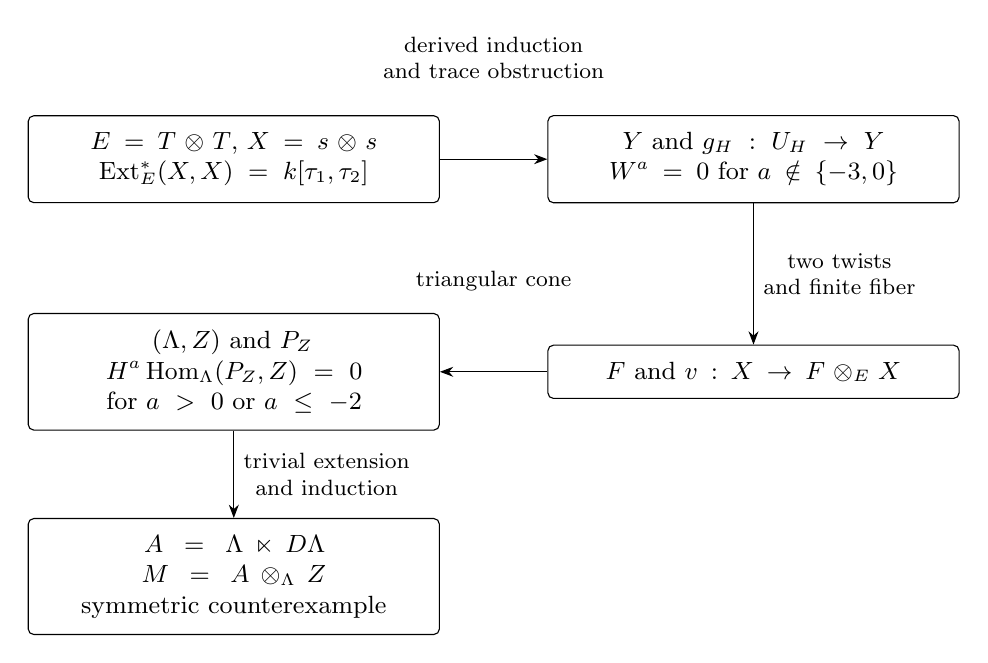
\begin{tikzpicture}[>=Stealth,
 box/.style={draw,rounded corners=2pt,align=center,text width=4.8cm,
             inner sep=6pt,font=\small},
 lab/.style={font=\footnotesize,align=center}]
\node[box] (ex) at (0,3.7)
 {$E=T\otimes T$, $X=s\otimes s$\\$\Ext_E^*(X,X)=k[\tau_1,\tau_2]$};
\node[box] (y) at (6.6,3.7)
 {$Y$ and $g_H:U_H\to Y$\\$W^a=0$ for $a\notin\{-3,0\}$};
\node[box] (fv) at (6.6,1)
 {$F$ and $v:X\to F\otimes_E X$};
\node[box] (lz) at (0,1)
 {$(\Lambda,Z)$ and $P_Z$\\$H^a\Hom_\Lambda(P_Z,Z)=0$\\for $a>0$ or $a\leq-2$};
\node[box] (am) at (0,-1.6)
 {$A=\Lambda\ltimes D\Lambda$\\$M=A\otimes_\Lambda Z$\\symmetric counterexample};
\draw[->] (ex)--node[above=9mm,lab]{derived induction\\and trace obstruction}(y);
\draw[->] (y)--node[right,lab]{two twists\\and finite fiber}(fv);
\draw[->] (fv)--node[above=9mm,lab]{triangular cone}(lz);
\draw[->] (lz)--node[right,lab]{trivial extension\\and induction}(am);
\end{tikzpicture}
\caption{Constructions and implications in the proof. The complete
self-Hom vanishing for $(\Lambda,Z)$ supplies the hypotheses for
transfer to $(A,M)$. Arrows indicate proof stages, not algebra maps.}
\label{fig:proof-architecture}
\end{figure}

\paragraph{Homological consequences.}
The pair $(A,M)$ gives counterexamples to several conjectures formulated
through injective resolutions and tilting modules. Corollary~\ref{cor:homological}
realizes five such failures using one endomorphism algebra and two
associated modules. We state the relevant conjectures in their
finite-dimensional left-module forms before giving the corollary.
For a finite-dimensional algebra $\Gamma$, write
\[
 0\longrightarrow {}_\Gamma\Gamma\longrightarrow I^0
 \longrightarrow I^1\longrightarrow\cdots
\]
for its minimal injective resolution. Its \emph{dominant dimension} is
the supremum of the integers $d\geq0$ for which $I^j$ is projective
whenever $0\leq j<d$, and is infinite when every $I^j$
is projective. The classical \emph{Nakayama conjecture} asserts that
infinite dominant dimension forces self-injectivity.
The \emph{generalized Nakayama conjecture} asserts that every
indecomposable injective occurs as a summand of some $I^j$; equivalently,
for every simple module $S$, some $\Ext_\Gamma^i(S,\Gamma)$ with
$i\geq0$ is nonzero. The \emph{strong Nakayama conjecture} asserts
that a finite module $V$ with $\Ext_\Gamma^i(V,\Gamma)=0$ for all
$i\geq0$ is zero. The \emph{Auslander--Gorenstein conjecture} asserts
that the bounds $\pd_\Gamma I^j\leq j$ for every $j\geq0$ force
finite self-injective dimension on both sides. These formulations are
recalled in~\cite[Introduction]{Zhang2018HomologicalConjectures}.

Write $\add W$ for the direct summands of finite direct sums of a
module $W$. A finite left $\Gamma$-module $W$ is \emph{tilting} if it
has finite projective dimension, is self-orthogonal, and admits a
finite exact coresolution
\[
 0\longrightarrow\Gamma\longrightarrow W^0\longrightarrow\cdots
 \longrightarrow W^r\longrightarrow0,\qquad W^j\in\add W.
\]
It is \emph{Wakamatsu tilting} if it is self-orthogonal and admits an
exact coresolution
\[
 0\longrightarrow\Gamma\longrightarrow W^0\longrightarrow W^1
 \longrightarrow\cdots,\qquad W^j\in\add W,
\]
which remains exact after applying $\Hom_\Gamma(-,W)$. This is the
finite left-module definition in~\cite[Definition~2.1]{Huang2006}.
The \emph{Wakamatsu tilting conjecture} asserts that a Wakamatsu tilting
module of finite projective dimension is tilting; see
\cite{DivaaniAazarMahinFallahTousi2025} for a recent discussion.

\begin{corollary}[Homological conjectures]\label{cor:homological}
Let $A,M$ be as in Theorem~\ref{thm:main}. For every field extension
$K/k$, put $A_K=K\otimes_k A$, $M_K=K\otimes_k M$, and
\[
 \Gamma_K=\End_{A_K}(A_K\oplus M_K)^{\mathrm{op}}.
\]
Then $\Gamma_K$ is a finite-dimensional $K$-algebra with the following
properties, in the category of finite left $\Gamma_K$-modules.
\begin{enumerate}
\item Every term of the minimal injective resolution of $\Gamma_K$
is projective, but $\idim_{\Gamma_K}\Gamma_K=\infty$.
\item There is a nonzero simple module $S$ such that
$\Ext_{\Gamma_K}^i(S,\Gamma_K)=0$ for every $i\geq0$.
\item There is a projective-injective Wakamatsu tilting module $W$
which is not tilting.
\end{enumerate}
Consequently the classical, generalized, and strong Nakayama conjectures,
the Auslander--Gorenstein conjecture, and the Wakamatsu tilting conjecture
are false for finite-dimensional algebras over $K$.
\end{corollary}

The opposite in this definition keeps our left-module convention. The
endomorphism-algebra connection with dominant dimension is classical,
going back to Mueller~\cite[Lemma~3 and Theorem~4]{Mueller1968}; the precise
Tachikawa--Nakayama correspondence for a pair $(A,M)$ is also stated
in~\cite[p.~7288]{ChenXi2025TAMS}. Section~\ref{sec:consequences}
uses this connection and constructs the modules $S$ and $W$ directly.
Taking $K$ to be an algebraic closure of $k$ gives examples over an
algebraically closed field of characteristic two. This field contains
the displayed transcendental parameters; the assertion does not concern
the algebraic closure of a finite field.

The same resolution also gives a finitistic-dimension consequence.
For a finite-dimensional algebra, the \emph{little left finitistic
dimension} is the supremum of the finite projective dimensions of
finite left modules; the \emph{big left finitistic dimension} allows
all left modules instead.

\begin{corollary}[Finitistic dimensions]\label{cor:finitistic}
Let $k$ be the field in Theorem~\ref{thm:main}, let $K/k$ be any field
extension, and let $\Gamma_K$ be the algebra in
Corollary~\ref{cor:homological}. For every integer $n\geq1$, there is a
finite-dimensional left $\Gamma_K$-module $C_n$ such that
\[
 \pd_{\Gamma_K}C_n=n.
\]
Consequently $\Gamma_K$ has infinite little left finitistic dimension
and infinite big left finitistic dimension.
\end{corollary}

This gives an independent characteristic-two example alongside the
complex algebra of~\cite[Theorem~1.1]{OpenAIFinitistic2026}.

Two further applications are developed in
Section~\ref{sec:consequences}. The connection between generalized
Nakayama failure and cotilting complements established by Buan and Solberg
\cite[Theorems~3.1 and~3.4]{BuanSolberg1998} gives a projective module
over $\Gamma_K^{\mathrm{op}}$ that can be completed to a tilting module
in infinitely many ways, each by adjoining one indecomposable summand;
these summands are pairwise nonisomorphic
(Corollary~\ref{cor:tilting-complements}). Their introduction credits
an independent proof of this connection to Happel and Unger
\cite[Introduction]{BuanSolberg1998}. The mirror-reflective
constructions of Chen, Fang and Xi~\cite{ChenFangXi2024} give auxiliary
indecomposable symmetric algebras with arbitrarily long idempotent
stratifications and the resulting chains of successive derived-category
recollements specified in Corollary~\ref{cor:stratifying}.

\paragraph{Organization.}
Section~\ref{sec:homological} establishes the complete-resolution,
duality, and finite-representative tools.
Section~\ref{sec:transfer} proves the transfer to a symmetric algebra.
Sections~\ref{a:section} and~\ref{e:section} construct the starting
algebra and compute the stable self-maps and twist actions.
Section~\ref{b:section} constructs the finite bimodule and proves the
trace obstruction. Section~\ref{sec:triangular} forms the triangular
module, establishes the complete vanishing profile, and applies the
transfer to prove Theorem~\ref{thm:main}.
Section~\ref{sec:consequences} studies the associated endomorphism
algebra and proves Corollaries~\ref{cor:homological} and~\ref{cor:finitistic}.

\paragraph{Conventions.}
All algebras are associative and unital, all modules are unital left
modules unless indicated otherwise, and all modules occurring in the
construction are finite-dimensional.
Unspecified tensor products are over $k$, and
$G^e=G\otimes_k G^{\mathrm{op}}$ acts on $G$-bimodules by the usual
outer actions.  Complexes are indexed homologically, with
$P[a]_j=P_{j-a}$.  Since the field has characteristic two, signs in
their differentials and comparison maps disappear.  The following
section fixes the stable and derived conventions used throughout.

\section{Homological preliminaries}\label{sec:homological}

The tools in this section serve two passages in the construction.
Complete-resolution comparison will turn the triangular cone's
endomorphism calculation into the vanishing needed for transfer to a
symmetric algebra. Stable duality will supply the negative-degree maps
used in that calculation. Separately, projective models and their stable
images will turn the derived-induction object into a finite bimodule,
preserving its maps and connecting morphisms under evaluation.

Throughout the construction, $k$ has characteristic two. Unless explicitly
stated otherwise, algebras and modules are finite dimensional over $k$.
Resolution and model complexes have finite-dimensional terms; the full Hom
complexes defined below may have infinite-dimensional product terms.
Modules are left modules unless a side is specified. Write
$D=\Hom_k(-,k)$ and $G^e=G\otimes_kG^{\mathrm{op}}$; an unsubscripted tensor
product is over $k$. Differentials lower homological degree, and
\[
 P[a]_j=P_{j-a},\qquad c_jP=\coker(d^P_{j+1}:P_{j+1}\longrightarrow P_j).
\]
Characteristic two removes the signs in shifts, tensor differentials and cones.
For two complexes we use the full Hom complex
\begin{equation}\label{h:full-hom}
 \Hom_G^a(P,Q)=\prod_{j\in\mathbb Z}\Hom_G(P_j,Q_{j-a}),\qquad
 (\delta f)_j=d^Q_{j-a}f_j+f_{j-1}d^P_j.
\end{equation}
For a module $N$, viewed in degree zero, $\Hom_G(P,N)^a=\Hom_G(P_a,N)$.
The space $\sHom_G(M,N)$ is the quotient of $\Hom_G(M,N)$ by maps factoring
through finite projectives.

\subsection{Complete resolutions and stable duality}

An exact complex $P$ of projectives is \emph{totally acyclic} if
$\Hom_G(P,G)$ is exact. If $c_0P=M$, we call $P$ a complete resolution of $M$.
The comparison below also applies when $G$ is not self-injective.
Complete resolutions and passage from derived objects to stable modules
belong to the framework developed by Buchweitz~\cite{Buchweitz2021}.
We give the comparison and truncation arguments in our conventions.

\begin{lemma}[Complete-resolution comparison]\label{h:comparison}
Let $P$ be totally acyclic and let $Q$ be an exact complex of projectives.
For every integer $a$ there are natural isomorphisms
\begin{equation}\label{h:comparison-formula}
 H^a\Hom_G^\bullet(P,Q)
 \simeq\sHom_G(c_aP,c_0Q)
 \simeq H^a\Hom_G(P,c_0Q).
\end{equation}
The first isomorphism is induced by cokernels of shifted chain maps and
respects composition. For $a>0$ these spaces are
$\Ext_G^a(c_0P,c_0Q)$.
\end{lemma}

\begin{proof}
We first record the extension property supplied by total acyclicity. If $J$
is projective, then $\Hom_G(P,J)$ is exact, since $J$ is a summand of a finite
sum of copies of $G$. Identify $c_jP$ with $\im d_j^P\subset P_{j-1}$.
For $u:c_jP\to J$, the map $u d_j^P:P_j\to J$ is a cocycle.
Exactness gives $h:P_{j-1}\to J$ with $h d_j^P=u d_j^P$, so $h$ extends $u$.
It follows at once that the cycles of $\Hom_G(P,N)^a$ are maps
$c_aP\to N$ and its boundaries are exactly the maps factoring through
projectives. This proves the second isomorphism, with $N=c_0Q$.

For the first, begin in degree zero. A map $c_0P\to c_0Q$ lifts to
$f_0:P_0\to Q_0$, and then successively to $f_j$ for $j>0$, using
projectivity of $P_j$ and exactness of $Q$. To proceed downwards,
$d_j^Qf_j$ vanishes on $\ker d_j^P=\im d_{j+1}^P$ by the chain equation
already obtained in degree $j+1$. It therefore defines a map
$c_jP=\im d_j^P\to Q_{j-1}$. The extension property gives $f_{j-1}$.
Thus every cokernel map lifts to a full chain map.

A homotopy induces a projective factorization on $c_0$. Conversely, suppose
the cokernel map of $f$ factors as $c_0P\to J\to c_0Q$ with $J$ projective.
Extend its first factor to $P_{-1}$ and lift its second factor to $Q_0$.
Their composite is a homotopy component $h_{-1}:P_{-1}\to Q_0$ whose
homotopy differential removes the induced map on cokernels. It remains to
nullhomotope a chain map inducing zero there. For this remaining map set
$h_{-1}=0$. For $j\geq0$, lift
\[
 f_j+h_{j-1}d_j^P:P_j\longrightarrow\im d_{j+1}^Q
\]
to $h_j:P_j\to Q_{j+1}$; the initial image assertion is the vanishing on
$c_0$, and each later one follows from the preceding chain equation.
For $j<0$, the map $f_j+d_{j+1}^Qh_j$ kills $\im d_{j+1}^P$ by the equation
in degree $j+1$. It descends to $\im d_j^P$ and extends to
$h_{j-1}:P_{j-1}\to Q_j$ by the same extension property. These equations
give $f=dh+hd$ in every degree. The product in \eqref{h:full-hom} permits all
these components; each equation uses only two of them.

Replace $P$ by $P[-a]$ to obtain degree $a$. The construction by cokernels
preserves compositions and shifts. Finally, the nonnegative tail of $P$
resolves $c_0P$. In every positive cohomological degree its Hom complex has
the same two adjacent differentials as $\Hom_G(P,c_0Q)$, proving the Ext
assertion, including degree one.
\end{proof}

Recall that $G$ is \emph{symmetric} if there is a bimodule isomorphism
$G\simeq DG$, or equivalently a linear form $t:G\to k$ such that
$t(ab)=t(ba)$ and $(a,b)\mapsto t(ab)$ is nondegenerate. In this case finite
projectives are injective, and every finite module embeds in a finite
projective: dualize a finite projective surjection onto its dual.
Splicing a projective resolution and a projective-injective coresolution
therefore gives a complete resolution of every finite module; applying
$\Hom_G(-,G)$ preserves its exactness because $G$ is injective.

For such a resolution put $M[a]=c_{-a}P$ in the stable category. The exact
sequences
\begin{equation}\label{h:syzygy-sequence}
 0\longrightarrow c_{j+1}P\longrightarrow P_j
 \longrightarrow c_jP\longrightarrow0
\end{equation}
show that $[1]$ is inverse syzygy. Lemma~\ref{h:comparison} makes these
shifts independent of choices, functorial on stable maps, and compatible
with composition. In particular,
\begin{equation}\label{h:stable-ext}
 H^a\Hom_G(P,N)=\sHom_G(M,N[a])\qquad(a\in\mathbb Z).
\end{equation}
For positive degrees the shifted composition is the Yoneda product, since
both are computed by lifting maps to projective resolutions.

A short exact sequence $0\to L\to V\to N\to0$ gives a long exact sequence
of the groups in \eqref{h:stable-ext}: apply $\Hom_G(P,-)$ termwise.
Its connecting map is composition with $\partial:N\to L[1]$. Concretely,
lift a projective surjection $J\to N$ to $J\to V$ and restrict to its kernel.
The resulting map $\Omega N\to L$, shifted once, is $\partial$.
This agrees with the cochain connecting map, which lifts a cocycle and
then applies the differential. We use this description to keep track of
connecting maps, as well as the groups in the long exact sequences.

The next lemma is the symmetric form of Auslander--Reiten duality,
also called Tate duality; see
\cite[Section~2, (2.3) and (2.7)--(2.8)]{Linckelmann2013}.
Its composition pairing will determine the action on negative-degree
self-maps.

\begin{lemma}[Symmetric stable duality]\label{h:duality}
For a symmetric algebra $G$ there are natural isomorphisms
\begin{equation}\label{h:duality-formula}
 D\sHom_G(M,N)\simeq\sHom_G(N,M[-1]).
\end{equation}
There is a linear functional $\lambda_M:\sHom_G(M,M[-1])\to k$ for which
the perfect pairing is $(f,g)\mapsto\lambda_M(gf)$. Consequently, for every
integer $a$ the pairing
\begin{equation}\label{h:shifted-pairing}
 \sHom_G(M,N[a])\times\sHom_G(N,M[-a-1])\longrightarrow k,
 \qquad (\alpha,\beta)\longmapsto\lambda_M\bigl(\beta[a]\alpha\bigr)
\end{equation}
is perfect and natural.
\end{lemma}

\begin{proof}
For every finite projective $J$ the finite-dimensional adjunction gives
\[
 D\Hom_G(J,N)\simeq\Hom_G(N,DG\otimes_GJ)\simeq\Hom_G(N,J).
\]
The first identification is immediate for $J=G$, hence for finite sums
and summands; the second uses a fixed symmetrizing form. Apply this
termwise to a complete resolution $P$ of $M$. Dualizing degree-zero
cohomology of $\Hom_G(P,N)$ yields
\[
 \frac{\Hom_G\bigl(N,\ker(P_0\to P_{-1})\bigr)}
 {\im\bigl(\Hom_G(N,P_1)\to
                \Hom_G(N,\ker(P_0\to P_{-1}))\bigr)}.
\]
Here $\ker(P_0\to P_{-1})=c_1P=M[-1]$. A factorization through any
projective lifts through $P_1\twoheadrightarrow c_1P$, so the displayed
quotient is precisely $\sHom_G(N,M[-1])$. All identifications are natural;
comparison of complete resolutions also gives naturality in $M$.

Define $\lambda_M(g)$ by pairing $1_M$ with $g$. Naturality in $N$, applied
to $f:M\to N$, identifies the pairing of $f$ and $g$ with
$\lambda_M(gf)$. Replacing $N$ by $N[a]$ and using the shift equivalences
gives \eqref{h:shifted-pairing}.
\end{proof}

\subsection{Projective models and their stable images}

In Section~\ref{b:section}, derived induction first supplies a bounded
derived bimodule. We will obtain the finite bimodule $Y$ from high
cokernels of a projective model. To compute its evaluated stable Hom
groups, we must also retain the actual maps attaching the model's
successive pieces. The next two lemmas establish this passage from
derived objects and connecting morphisms to finite stable modules.

We write $\mathrm D^b(G)$ for the derived category of bounded complexes of
finite modules. A complex is \emph{perfect} if it is derived isomorphic to
a bounded complex of finite projectives. We will represent bounded derived
objects by bounded-below complexes of finite projectives with bounded
homology. The following elementary facts specify the models and maps we use.
For a chain map $f:L\to N$, our cone convention is
\begin{equation}\label{h:cone}
 \Cone(f)_j=N_j\oplus L_{j-1},\qquad
 d_j^{\Cone(f)}=
 \begin{pmatrix}d_j^N&f_{j-1}\\0&d_{j-1}^L\end{pmatrix}.
\end{equation}

The projective-model statement is the bounded case of the standard
$K$-projective formalism; see
\cite[Proposition~1.4 and Example~3.2(a)]{Spaltenstein1988}, with the
opposite indexing convention for complexes.

\begin{lemma}[Derived maps and two-cell models]\label{h:derived-models}
A bounded-below complex $P$ of projectives computes derived maps out of it
by chain maps modulo homotopy. Every bounded complex of finite modules has
such a projective model with finite terms. In particular, two such models
of the same derived object are homotopy equivalent.

Suppose a derived triangle is given by
\[
 L\longrightarrow V\longrightarrow R\xrightarrow{\partial}L[1].
\]
For projective models $P_L,P_R$ and a chain map
$b:P_R\to P_L[1]$ representing $\partial$, a model of $V$ is the two-cell
complex
\begin{equation}\label{h:two-cell}
 P_{V,j}=P_{L,j}\oplus P_{R,j},\qquad
 d_j^{P_V}=\begin{pmatrix}d_j^{P_L}&b_j\\0&d_j^{P_R}\end{pmatrix}.
\end{equation}
Its subcomplex and quotient represent $L$ and $R$, and its connecting
map is the specified $\partial$.
\end{lemma}

\begin{proof}
Every chain map from $P$ to an acyclic complex is nullhomotopic: start at
the lowest nonzero degree of $P$ and successively lift the residual map
through the next differential of the target. The same argument applies
to every shift. Thus the full Hom from $P$ sends quasi-isomorphisms to
quasi-isomorphisms, which proves the assertion about derived maps. This is
the $K$-projectivity of a bounded-below projective source; it does not assert
$K$-projectivity of a complete resolution.

For completeness, a bounded-below finite complex $V$ admits a projective
model $\theta:Q\to V$ by the following induction. Having constructed lower
terms, choose $Q_j$ finite projective surjecting onto
\[
 \{(x,y)\in V_j\oplus Q_{j-1}:d_Vx=\theta(y),\ d_Qy=0\}.
\]
Use its two components for $\theta_j$ and $d_j^Q$. Every cycle of the
comparison cone is then a boundary, so $\theta$ is a quasi-isomorphism.
A derived isomorphism between projective models and its inverse are
represented by chain maps, and their composites are homotopic to the
identities by the first assertion.

To verify the last assertion, represent the first arrow of the triangle
by $f:P_L\to P_V$ on any projective models. Its cone represents $R$, and
the projection $\Cone(f)\to P_L[1]$ represents $\partial$.
The cone of the deshifted projection has $P_V$ as a subcomplex with
contractible quotient $\Cone(1_{P_L})$. It therefore represents $V$.
Replacing the projective models by homotopy equivalent ones and the map
by its prescribed representative preserves this conclusion: a homotopy
commuting square induces a cone map with that homotopy as its off-diagonal
component, and homotopic maps have isomorphic cones. The resulting cone
$\Cone(b[-1])$ is exactly \eqref{h:two-cell}.
\end{proof}

A bounded-below complex with bounded homology represents a bounded derived
object by good truncation. Also, a bounded complex whose terms have finite
projective dimension is perfect: its finite filtration by terms expresses
it as successive cones of shifts of modules with bounded projective
resolutions. These observations allow us to use the preceding models
without introducing infinite-dimensional terms.

\begin{lemma}[Stable images]\label{h:stable-image}
Let $G$ be symmetric and let $P$ be bounded below with projective terms and
bounded homology. For $n$ sufficiently large the formula
\begin{equation}\label{h:stable-image-formula}
 \langle P\rangle=(c_nP)[n]
\end{equation}
defines a stable module, independent of $n$ up to natural stable
isomorphism. It is functorial on derived maps represented by such models,
commutes with shifts, sends a module to its stable class, and sends an Ext
class to its corresponding stable map.

A degreewise split short exact sequence $0\to P_L\to P_V\to P_R\to0$
of these complexes gives a stable connecting map
$\langle P_R\rangle\to\langle P_L\rangle[1]$ and the associated long exact
stable Hom sequences. With respect to a graded splitting, this connecting
map is the stable image of the cross differential
$b:P_R\to P_L[1]$ in \eqref{h:two-cell}.
\end{lemma}

\begin{proof}
Above the homology support, \eqref{h:syzygy-sequence} is exact for $P$.
It identifies $(c_{n+1}P)[n+1]$ with $(c_nP)[n]$, naturally on chain maps.
A homotopy changes $c_n(f)$ by a map factoring through $P_{n-1}$, so the
construction descends to homotopy classes. Lemma~\ref{h:derived-models}
then makes it functorial on derived maps. The identity
$c_n(P[a])=c_{n-a}P$ gives shift compatibility. A projective resolution of
a module recovers its successive syzygies, proving the assertion for
modules. Restricting a lifted representative of an Ext class to high
degrees gives the same successive syzygies of that map, proving the last
assertion about classes.

Choose $n$ so that all three complexes are exact in degrees at least $n$.
Their cokernels give a short exact sequence
\[
 0\longrightarrow c_nP_L\longrightarrow c_nP_V
 \longrightarrow c_nP_R\longrightarrow0.
\]
For injectivity on the left, suppose
$(x,0)=d_{n+1}^{P_V}(u,v)$. Then $d_{n+1}^{P_R}v=0$, so
$v=d_{n+2}^{P_R}w$ for some $w$. The equation $d_Lb+bd_R=0$ gives
$x=d_{n+1}^{P_L}(u+b_{n+2}w)$, as required. Surjectivity and exactness in
the middle follow by lifting components in the graded splitting.

There is a commutative diagram with exact rows
\[
\begin{tikzcd}[column sep=large]
0\arrow[r]&c_{n+1}P_R\arrow[r]\arrow[d,"\overline b_{n+1}"']
 &P_{R,n}\arrow[r]\arrow[d]
 &c_nP_R\arrow[r]\arrow[d,equal]&0\\
0\arrow[r]&c_nP_L\arrow[r]&c_nP_V\arrow[r]&c_nP_R\arrow[r]&0.
\end{tikzcd}
\]
The middle vertical map sends $z$ to the class of $(0,z)$. On an element
$d_{n+1}^{P_R}z$, its value is the class of $(b_{n+1}z,0)$, since
$(b_{n+1}z,d_{n+1}^{P_R}z)$ is a boundary in $P_V$. Thus the left vertical
map is induced by $b_{n+1}:P_{R,n+1}\to P_{L,n}$.
Shifting the left vertical arrow by $[n+1]$ gives
$\langle P_R\rangle\to\langle P_L\rangle[1]$. By the description after
\eqref{h:stable-ext}, this is the connecting map of the bottom row shifted
by $[n]$, and it is exactly $\langle b\rangle$. This also gives the
asserted long exact sequences.
\end{proof}

The following criterion supplies the other use of stable images in
Section~\ref{b:section}. There, an ordinary trace will rule out a perfect
factorization of a derived map. The criterion then shows that its stable
image is nonzero.

\begin{lemma}[Vanishing stable image and perfect factorization]
\label{h:perfect-factor}
Over a symmetric algebra, a derived map between bounded derived objects
whose stable image is zero factors in the derived category through a
perfect complex.
\end{lemma}

\begin{proof}
Choose bounded-below projective models $P,Q$ and represent the map by a
global chain map $f:P\to Q$, using Lemma~\ref{h:derived-models}. For a
sufficiently high $n$, both complexes are exact in degrees at least $n$
and $c_n(f)$ factors through a finite projective $J$:
\[
 c_nP\xrightarrow{u}J\xrightarrow{v}c_nQ.
\]
Since $J$ is injective, extend $u$ across
$c_nP=\im d_n^P\subset P_{n-1}$. Since $J$ is projective, lift $v$ to $Q_n$.
The composite gives $h_{n-1}:P_{n-1}\to Q_n$. It makes
$f_n+h_{n-1}d_n^P$ zero after projection to $c_nQ$, so this residual map
lifts through $d_{n+1}^Q$ to $h_n:P_n\to Q_{n+1}$. Inductively, for $j>n$
the chain equation and the preceding homotopy equation show that
$f_j+h_{j-1}d_j^P$ lands in $\ker d_j^Q=\im d_{j+1}^Q$. Lift it to $h_j$.
Set $h_j=0$ for $j<n-1$.

The homotopic map $f'=f+dh+hd$ now vanishes in every degree $j\geq n$.
Its chain equation in degree $n$ reads
\begin{equation}\label{h:truncation-boundary}
 f'_{n-1}d_n^P=0.
\end{equation}
Consequently its remaining components define a chain map into the actual
homological subcomplex $Q_{\leq n-1}$, obtained by retaining $Q_j$ for
$j\leq n-1$ and setting the higher terms to zero. Equation
\eqref{h:truncation-boundary} verifies the boundary condition at the cut.
Thus $f'$ factors through $Q_{\leq n-1}$, which is bounded and projective
because $Q$ was bounded below. Composing with the chosen model maps gives
the desired derived factorization. This also covers a map with a module
as target: first lift it globally to a projective resolution of that
module, and then apply this argument.
\end{proof}

\subsection{Bimodule evaluation}

For a symmetric algebra $E$, the tensor product of symmetrizing forms makes
$E^e$ symmetric. We call an $E$-bimodule \emph{side-projective} if it is
projective as a left and as a right $E$-module, and write $LX=L\otimes_EX$.
Side-projectivity does not assert projectivity over $E^e$.
For the derived-induction construction, the passage to a finite stable
bimodule must commute with evaluation at $X$, including the attaching
maps just discussed. The next lemma establishes these compatibilities.

\begin{lemma}[Finite shifts and evaluation]\label{h:evaluation}
Every stable shift of a finite side-projective bimodule has a finite
side-projective representative. Evaluation at a finite $E$-module $X$
sends stable maps between these bimodules to stable $E$-module maps and
has natural identifications
\begin{equation}\label{h:evaluation-shifts}
 (L[a])X\simeq(LX)[a],\qquad L(X[a])\simeq(LX)[a].
\end{equation}
It preserves the stable connecting maps of short exact sequences of
side-projective bimodules, and these identifications are natural in both
$L$ and $X$.

If $P$ is a bounded-below complex of projective bimodules with bounded
homology and all sufficiently high $c_nP$ are side-projective, then
$P\otimes_EX$ has bounded homology and
\begin{equation}\label{h:evaluation-image}
 \langle P\rangle X\simeq\langle P\otimes_EX\rangle,
\end{equation}
naturally on maps and on connecting maps from degreewise split sequences
of such complexes. The hypothesis on the high cokernels holds whenever
$P$, considered separately on either side, is homotopy equivalent to a
bounded complex of projectives on that side.
\end{lemma}

\begin{proof}
Take a projective bimodule surjection onto $L$. Its kernel is
side-projective because the sequence splits on each side. For a positive
shift, use the finite projective-injective embedding
\[
 L\longrightarrow\Hom_k(E^e,L),\qquad
 z\longmapsto(a\longmapsto az),
 \qquad (r\varphi)(a)=\varphi(ar).
\]
Its target is injective by coinduction and projective by symmetry of
$E^e$. The embedding splits on each side because $L$ is injective on
that side, so its cokernel is again side-projective. Iteration supplies
finite representatives for every shift.

An $E^e$-projective evaluates to an $E$-projective: this is immediate for
the free bimodule $E\otimes E$, which evaluates to $E\otimes X$, and
passes to finite sums and summands. Hence evaluation respects projective
factorizations. Every short exact sequence of side-projective bimodules
splits on the right, and therefore remains exact after evaluation. In
particular, evaluating the sequences just used to define shifts gives
the first identification in \eqref{h:evaluation-shifts}. Applying the
projective-presentation description of connecting maps to these same
sequences shows that their actual connecting maps are preserved.

For fixed $L$, right projectivity makes $L\otimes_E-$ exact, and left
projectivity makes it preserve projectives. Applying it to projective
resolutions and projective-injective coresolutions gives the second
identification in \eqref{h:evaluation-shifts}. A bimodule map $L\to L'$
gives a natural transformation on these complexes; thus evaluating it
on a shifted module agrees stably with shifting its evaluation. The
same reasoning proves naturality in $X$ and compatibility with
composition.

For the complex assertion, the high exact sequences
$0\to c_{n+1}P\to P_n\to c_nP\to0$ split on the right. Their evaluations
remain exact, proving bounded homology of $P\otimes_EX$; its terms are
projective by the preceding argument. Right exactness gives the
canonical identifications
\[
 c_n(P\otimes_EX)=(c_nP)\otimes_EX.
\]
Together with \eqref{h:evaluation-shifts}, these identify the two sides
of \eqref{h:evaluation-image}. They commute with chain maps. For a
filtered complex, the cross differential in
Lemma~\ref{h:stable-image} evaluates to its tensor with $X$. That lemma's
explicit diagram therefore identifies the evaluated connecting map with
the connecting map after evaluation.

Finally, suppose a homotopy equivalence on one side compares $P$ with a
complex supported in degrees at most $d$. At any $n>d$, the homotopy
between the identity and the composite through that complex gives
\[
 1_{P_n}=d_{n+1}h_n+h_{n-1}d_n.
\]
Writing $\pi_n:P_n\to c_nP$, passage to the cokernel yields
\[
 1_{c_nP}=(\pi_nh_{n-1})\overline d_n,
 \qquad \overline d_n:c_nP\longrightarrow P_{n-1}.
\]
Thus $c_nP$ is a summand of a projective on that side. The separate
homotopy equivalence on the other side proves the other projectivity.
The homotopies need not be bimodule homotopies.
\end{proof}

\section{Passing to a symmetric algebra}\label{sec:transfer}

The final step of the construction has a general form.  It explains why
we will need vanishing in negative degrees as well as positive ones.
Throughout this section, $R$ is a finite-dimensional algebra over our
field $k$ and $D=\Hom_k(-,k)$.

We recall the standard symmetry of a trivial extension; see
\cite[Proposition~3.1]{BessenrodtHolmZimmermann2007}.

\begin{lemma}\label{tr:trivial-symmetric}
The trivial extension $R\ltimes DR$ is a finite-dimensional symmetric
algebra.  In particular, its left and right regular modules are
injective in the categories of all unital modules.
\end{lemma}

\begin{proof}
The dual bimodule structure is
\[
 (a\lambda b)(c)=\lambda(bca)
 \qquad(a,b,c\in R,\ \lambda\in DR),
\]
and the multiplication is
\[
 (a,\lambda)(b,\mu)=(ab,a\mu+\lambda b).
\]
The bimodule identities give associativity, and $(1,0)$ is a unit.
The functional $t(a,\lambda)=\lambda(1)$ gives the pairing
\[
 t\big((a,\lambda)(b,\mu)\big)=\mu(a)+\lambda(b).
\]
This pairing is symmetric and nondegenerate, and associativity of the
algebra makes it an associative form.  Thus $R\ltimes DR$ is isomorphic
to its dual as a bimodule.

For any algebra $G$ over $k$, the natural isomorphism
$\Hom_G(L,DG)\simeq\Hom_k(L,k)$ shows that $DG$ is an injective left
$G$-module; the same argument applies on the right.  This statement
holds for arbitrary unital $L$, since vector-space duality is exact.
Applying it to the symmetric algebra $G=R\ltimes DR$ proves the final
assertion.
\end{proof}

\begin{proposition}[Transfer through the trivial extension]
\label{tr:transfer}
Let $P$ be a totally acyclic complex of finite projective left
$R$-modules, and put $Z=c_0P$.  Suppose that $Z$ is nonprojective and
\begin{equation}\label{tr:two-sided-vanishing}
 H^a\Hom_R(P,Z)=0
 \qquad\text{for }a>0\text{ and for }a\leq -2.
\end{equation}
Then
\[
 A=R\ltimes DR,\qquad M=A\otimes_R Z
\]
are a finite-dimensional symmetric algebra and a finite-dimensional
nonprojective left $A$-module satisfying
\[
 \Ext_A^a(M,M)=0\qquad(a>0).
\]
\end{proposition}

\begin{proof}
Write $\nu=DR\otimes_R-$ and set $I=\nu P$.  Finite projectivity gives
natural isomorphisms
\begin{equation}\label{tr:nakayama-evaluation}
 DR\otimes_R P_j\simeq D\Hom_R(P_j,R),
 \qquad
 \Hom_R(Z,DR\otimes_R P_j)\simeq D\Hom_R(P_j,Z).
\end{equation}
Both follow first for finite free modules and then for their direct
summands.  The module $\Hom_R(P_j,R)$ is finite projective on the right,
so $I_j$ is injective on the left.  Total acyclicity of $P$ and exactness
of $D$ show that the entire complex $I$ is exact.

As a right $R$-module, $A=R\oplus DR$.  Consequently the restriction of
$A\otimes_RP$ is the exact complex $P\oplus I$.  Every term
$A\otimes_RP_j$ is finite projective over $A$, since induction preserves
a split direct-summand presentation.  Right exactness identifies
$c_0(A\otimes_RP)$ with $A\otimes_RZ=M$.  Thus the nonnegative tail of
$A\otimes_RP$ is a projective resolution of $M$.  In particular, the
tensor exactness needed here has been proved for this resolution;
flatness of $A_R$ is not an additional hypothesis.

Put $N=\nu Z$.  Again by right exactness, $N=c_0I$.  Exactness of $I$
identifies this cokernel with $\im(I_0\to I_{-1})$.  Hence
\begin{equation}\label{tr:injective-tail}
 0\longrightarrow N\longrightarrow I_{-1}
 \longrightarrow I_{-2}\longrightarrow I_{-3}\longrightarrow\cdots
\end{equation}
is an injective coresolution.  If $C^j=\Hom_R(P_j,Z)$ with differential
$\delta^j:C^j\to C^{j+1}$, applying $\Hom_R(Z,-)$ to
\eqref{tr:injective-tail} gives, in cohomological degrees $0,1,2$,
\[
 DC^{-1}\xrightarrow{D\delta^{-2}}DC^{-2}
 \xrightarrow{D\delta^{-3}}DC^{-3}.
\]
Both arrows surrounding degree one are present.  More generally, the
term in degree $a\geq0$ is $DC^{-a-1}$.  Thus, for every $a>0$,
\begin{equation}\label{tr:negative-duality}
 \Ext_R^a(Z,N)\simeq D H^{-a-1}\Hom_R(P,Z)=0.
\end{equation}
The first of these equalities uses degree $-2$, which accounts for the
endpoint in \eqref{tr:two-sided-vanishing}.

Induction--restriction adjunction on the projective resolution already
constructed now yields
\begin{align*}
 \Ext_A^a(M,M)
 &\simeq \Ext_R^a\bigl(Z,\Res_R^A M\bigr)\\
 &\simeq \Ext_R^a(Z,Z)\oplus\Ext_R^a(Z,N)=0
 \qquad(a>0).
\end{align*}
Here the first summand vanishes by
\eqref{tr:two-sided-vanishing} and Lemma~\ref{h:comparison}, and the
second by \eqref{tr:negative-duality}.

Lemma~\ref{tr:trivial-symmetric} proves that $A$ is symmetric.  The
module $M$ is finite and unital.  Finally, if $M$ were a direct summand
of $A^r$, tensoring the splitting with the quotient $A\to R$ would make
\[
 R\otimes_A M\simeq R\otimes_A(A\otimes_RZ)\simeq Z
\]
a direct summand of $R^r$.  A tensor functor preserves a split identity
composite without any flatness assumption.  This contradicts
nonprojectivity of $Z$.
\end{proof}

We will apply Proposition~\ref{tr:transfer} to a triangular algebra
$R=\Lambda$.  The rest of the proof constructs its module $Z$ together
with the complete resolution and the two vanishing ranges in
\eqref{tr:two-sided-vanishing}.

\section{The ten-dimensional algebra}
\label{a:section}

We now construct an algebra \(C\) and a simple module \(s\) whose
resolution supplies the degree-three extension classes used below.
Besides this resolution, we need
finite projective-dimension bounds for the dual regular modules;
these bounds make derived induction admit a finite bimodule
representative. The multiplication of $C$ is the one in
\cite[Section~4.1]{OpenAIAR2026}; all properties needed here are proved
directly.  We work over the fixed field
\(k=\mathbb F_2(q,H_1,H_2)\), where the three parameters are
algebraically independent.

Let \(C\) have the following basis, arranged by its left and right
idempotents:
\begin{equation}
\begin{array}{c|c@{\qquad}c|c}
\text{corner}&\text{basis}&\text{corner}&\text{basis}\\ \hline
eCe&e,x,y,z&eCf&u,v\\
fCe&t,j&fCf&f,n.
\end{array}
\label{a:corners}
\end{equation}
The unit is \(1=e+f\).  The complete multiplication table, with the
left factor indexing the row, is
\begin{equation}
\begingroup
\setlength{\arraycolsep}{4pt}
\begin{array}{c|cccccccccc}
 &e&f&x&y&z&u&v&t&j&n\\ \hline
e&e&0&x&y&z&u&v&0&0&0\\
f&0&f&0&0&0&0&0&t&j&n\\
x&x&0&0&qz&0&v&0&0&0&0\\
y&y&0&z&0&0&v&0&0&0&0\\
z&z&0&0&0&0&0&0&0&0&0\\
u&0&u&0&0&0&0&0&y+qx&z&v\\
v&0&v&0&0&0&0&0&qz&0&0\\
t&t&0&j&q^2j&0&(1+q)n&0&0&0&0\\
j&j&0&0&0&0&0&0&0&0&0\\
n&0&n&0&0&0&0&0&qj&0&0
\end{array}
\endgroup
\label{a:multiplication}
\end{equation}

\begin{lemma}\label{a:table}
The table \eqref{a:multiplication} defines an associative unital algebra
of dimension ten.  Its radical is the span of the eight basis vectors
other than \(e,f\), and \((\rad C)^5=0\).
\end{lemma}

\begin{proof}
Give the basis vectors the degrees
\[
\begin{gathered}
\deg e=\deg f=0,\qquad \deg u=\deg t=1,\\
\deg x=\deg y=\deg n=2,\qquad
\deg v=\deg j=3,\qquad \deg z=4.
\end{gathered}
\]
The table is homogeneous and respects the corners.  Thus associativity
with an idempotent, or with incompatible adjacent corners, follows
from \eqref{a:corners}.  For positive-degree triples of total degree
greater than four, both bracketings vanish.  The remaining composable
triples and the value of either bracketing are precisely
\[
\begin{array}{c|ccccc}
abc&utu&tut&xut&yut&ntu\\ \hline
(ab)c=a(bc)&(1+q)v&q(1+q)j&qz&qz&0
\end{array}
\]
\[
\begin{array}{c|cccccc}
abc&unt&txu&tyu&utx&uty&tun\\ \hline
(ab)c=a(bc)&qz&0&0&z&q^2z&0.
\end{array}
\]
Every entry is obtained by two applications of
\eqref{a:multiplication}; this exhausts the associativity check by
trilinearity.  The positive-degree span is a nilpotent ideal with
fifth power zero and quotient \(ke\oplus kf\cong k^2\).  It is therefore
the radical.
\end{proof}

Let \(s\) be the one-dimensional left \(C\)-module on which \(f\)
acts as the identity and every other basis vector acts as zero.
Its vector space dual \(Ds\) is the right simple with the same character.

The corner \(eCe\) gives a concrete connection with Schulz's
example~\cite[Example~7]{Schulz1995}. The table identifies it with
the quantum exterior algebra
\[
 eCe\cong k\langle x,y\rangle/(x^2,y^2,yx-q^{-1}xy).
\]
Moreover, the assignments
\(t\mapsto x+q^{-1}y\) and \(j\mapsto q^{-1}z\) give an
isomorphism of right \(eCe\)-modules
\[
 fCe\cong(x+q^{-1}y)eCe.
\]
The identities \(tx=j\), \(ty=q^2j\), and \(jx=jy=0\) verify
right-linearity, and the two images form a basis of the right ideal.
With Schulz's
parameter \(p=q^{-1}\), this right ideal is the first syzygy of his
module \((x+y)eCe\). The later left-module resolutions will use the
same type of parameter shift within the ten-dimensional algebra.

Write \(a^*\) for the basis vector of \(DC\) dual to a basis vector
\(a\) of \(C\).  Form the trivial extension
\begin{equation}
T=C\ltimes DC,\qquad
(a,\phi)(b,\psi)=(ab,a\psi+\phi b),\qquad
(a\phi b)(c)=\phi(bca).
\label{a:trivial-extension}
\end{equation}
By Lemma~\ref{tr:trivial-symmetric}, this is a symmetric algebra of
dimension twenty, with symmetrizing functional
\(t_T(a,\phi)=\phi(1)\).  In particular,
\[
t_T\bigl((a,\phi)(b,\psi)\bigr)=\phi(b)+\psi(a).
\]
We regard \(s\) as a \(T\)-module through the quotient \(T\to C\).
Set
\begin{equation}
B=C\otimes C\subseteq E=T\otimes T.
\label{a:tensor-algebras}
\end{equation}
Then \(\dim_k B=100\) and \(\dim_k E=400\).  The functional
\(t_E=t_T\otimes t_T\) gives a symmetric nondegenerate product pairing,
so \(E\) is symmetric.

We record the radical and corner information that will enter the trace
argument.  One has
\begin{align}
\rad T&=(\rad C)\oplus DC,\nonumber\\
\rad B&=(\rad C)\otimes C+C\otimes(\rad C),\nonumber\\
\rad E&=(\rad T)\otimes T+T\otimes(\rad T).
\label{a:radicals}
\end{align}
For the first equality, the displayed ideal is a square-zero extension
of the nilpotent ideal \(\rad C\), and its quotient is \(k^2\).
For the tensor products the displayed ideals are sums of commuting
nilpotent ideals, and their quotients are \(k^4\).  This proves all
three equalities.  The four vertex idempotents of \(B\), also used in
\(E\), are \(e\otimes e,e\otimes f,f\otimes e,f\otimes f\).
For these vertices the corner dimensions are
\begin{equation}
\bigl(\dim_k(pB p')\bigr)_{p,p'}=
\begin{pmatrix}
16&8&8&4\\
8&8&4&4\\
8&4&8&4\\
4&4&4&4
\end{pmatrix}.
\label{a:corner-parity}
\end{equation}
Indeed these dimensions are the products of the corresponding corner
dimensions \(4,2,2,2\) of \(C\).  In particular, every entry is even.

For \(i\in\mathbb Z\), put
\[
\ell_i=x+q^i y.
\]
We denote right multiplication by \(a\) by \(\rho_a\) and left
multiplication by \(a\) by \(\lambda_a\).  Thus \(\rho_a\) is a map
of left modules and \(\lambda_a\) is a map of right modules whenever
the indicated source and target corners allow it.

\begin{proposition}\label{a:dual-dimensions}
The dual regular module \(DC\) has projective dimension at most two
on both sides.  More precisely,
\[
D(eC)\cong Ce,\qquad D(Ce)\cong eC,
\]
and there are exact sequences
\begin{align}
0\longrightarrow Cf\xrightarrow{\rho_t}Ce
 \xrightarrow{\rho_{\ell_{-2}}}Ce
 \xrightarrow{e\mapsto j^*}D(fC)\longrightarrow0,
\label{a:left-dual-resolution}\\
0\longrightarrow fC\xrightarrow{\lambda_u}eC
 \xrightarrow{\lambda_{\ell_0}}eC
 \xrightarrow{e\mapsto v^*}D(Cf)\longrightarrow0.
\label{a:right-dual-resolution}
\end{align}
Consequently
\begin{equation}
\pd_B({}_B E)\le4,\qquad
\pd_{B^{\mathrm{op}}}(E_B)\le4,\qquad
\idim_B({}_B B)\le4.
\label{a:dimension-bounds}
\end{equation}
\end{proposition}

\begin{proof}
The pairing \(eC\times Ce\to k\) that takes the coefficient of \(z\)
in a product is nondegenerate.  In the ordered bases
\[
\mathcal B_{eC}=(e,x,y,z,u,v),\qquad
\mathcal B_{Ce}=(e,x,y,z,t,j),
\]
its only nonzero entries are the products
\(ez,xy,yx,ze,uj,vt\), with coefficients \(1,q,1,1,1,q\).
Thus it has determinant \(q^2\ne0\).  The maps sending \(e\) to
\(z^*\) give the stated left- and right-module isomorphisms.

Here is the full calculation for the other dual summands.  The two
surjections, on the ordered bases just specified, have the images
\begin{align*}
Ce\longrightarrow D(fC):\quad
(e,x,y,z,t,j)&\longmapsto
(j^*,t^*,q^2t^*,0,qn^*,f^*),\\
eC\longrightarrow D(Cf):\quad
(e,x,y,z,u,v)&\longmapsto
(v^*,u^*,u^*,0,n^*,f^*).
\end{align*}
Each has rank four; their kernels are respectively
\(\langle\ell_{-2},z\rangle_k\) and
\(\langle\ell_0,z\rangle_k\).
The intermediate maps have images and kernels
\[
\begin{array}{c|c|c}
\text{map}&\text{image}&\text{kernel}\\ \hline
\rho_{\ell_{-2}}:Ce\to Ce
 &\langle\ell_{-2},z\rangle_k
 &\langle y+qx,z,t,j\rangle_k\\
\lambda_{\ell_0}:eC\to eC
 &\langle\ell_0,z\rangle_k
 &\langle y+qx,z,u,v\rangle_k.
\end{array}
\]
For completeness, the initial injections are given by
\begin{align*}
\rho_t:(f,u,v,n)&\longmapsto(t,y+qx,qz,qj),\\
\lambda_u:(f,t,j,n)&\longmapsto(u,y+qx,z,v).
\end{align*}
Their four images are independent and span the respective kernels in
the table.  This proves exactness of
\eqref{a:left-dual-resolution} and
\eqref{a:right-dual-resolution}, including their orientations and
the exceptional index \(-2\) in the first sequence.

On either \(C\)-side, \(T=C\oplus DC\) has a projective resolution of
length at most two.  Tensor two such resolutions over the field and
totalize.  The resulting resolutions of the corresponding
\(B\)-modules \(E\) have length at most four, proving the first two
bounds in \eqref{a:dimension-bounds}.  Likewise
\(DB\cong DC\otimes DC\) has right \(B\)-projective dimension at most
four.  Dualizing a finite projective resolution gives an injective
coresolution of \({}_B B\), and proves the last bound.
\end{proof}

We now resolve \(s\). The same multiplication maps will also determine
the dual complex, including its right-module cohomology.

\begin{proposition}\label{a:resolution}
The augmentation \(Cf\to s\) extends to a projective resolution
\(R\to s\) with
\begin{equation}
R_0=Cf,\qquad R_i=Ce\ (i\ge1),\qquad
d_1=\rho_u,\qquad d_{i+2}=\rho_{\ell_i}\ (i\ge0).
\label{a:simple-resolution}
\end{equation}
It satisfies
\begin{equation}
H^a\Hom_C(R,s)=
\begin{cases}k&a=0,\\0&a\ne0,\end{cases}
\qquad
H^a\Hom_C(R,C)=
\begin{cases}Ds&a=2,\\0&a\ne2,\end{cases}
\label{a:dual-cohomology}
\end{equation}
where the second identification is an isomorphism of right
\(C\)-modules.
\end{proposition}

\begin{proof}
On the basis \((e,x,y,z,t,j)\) of \(Ce\), right multiplication gives
\begin{align*}
\rho_u(e,x,y,z,t,j)
  &=(u,v,v,0,(1+q)n,0),\\
\rho_{\ell_i}(e,x,y,z,t,j)
  &=(\ell_i,q^{i+1}z,z,0,(1+q^{i+2})j,0).
\end{align*}
For every \(i\ge0\), the coefficient \(1+q^{i+2}\) is nonzero.
Consequently
\[
\begin{array}{c|c|c}
\text{map}&\text{image}&\text{kernel}\\ \hline
\rho_u
 &\langle u,v,n\rangle_k
 &\langle\ell_0,z,j\rangle_k\\
\rho_{\ell_i},\ i\ge0
 &\langle\ell_i,z,j\rangle_k
 &\langle\ell_{i+1},z,j\rangle_k.
\end{array}
\]
The first image is \(\rad(Cf)\), and each later image is the preceding
kernel.  This proves exactness at every index.  Since
\(\Hom_C(Ce,s)=es=0\) and \(\Hom_C(Cf,s)=fs=k\), the first equality
in \eqref{a:dual-cohomology} follows.

Under \(\Hom_C(Cf,C)=fC\) and \(\Hom_C(Ce,C)=eC\), the dual cochain
complex is
\begin{equation}
fC\xrightarrow{\lambda_u}eC
 \xrightarrow{\lambda_{\ell_0}}eC
 \xrightarrow{\lambda_{\ell_1}}eC
 \xrightarrow{\lambda_{\ell_2}}\cdots,
\label{a:dual-complex}
\end{equation}
starting in degree zero.  The first arrow is injective, with image
\(\langle u,y+qx,z,v\rangle_k\).  For \(i\ge0\),
\[
\lambda_{\ell_i}(e,x,y,z,u,v)
  =(\ell_i,q^iz,qz,0,(1+q^i)v,0).
\]
The image and kernel are therefore
\[
\begin{array}{c|c|c}
 &\text{image}&\text{kernel}\\ \hline
i=0&\langle\ell_0,z\rangle_k
 &\langle\ell_{-1},z,u,v\rangle_k\\
i\ge1&\langle\ell_i,z,v\rangle_k
 &\langle\ell_{i-1},z,v\rangle_k.
\end{array}
\]
Since \(q\ell_{-1}=qx+y\), the first kernel equals the image of
\(\lambda_u\).  The only remaining cohomology is in degree two:
\[
\frac{\langle\ell_0,z,v\rangle_k}
     {\langle\ell_0,z\rangle_k}=k\overline v.
\]
Finally \(vf=v\), \(ve=0\), and the only nonzero product of \(v\)
with a radical basis vector is \(vt=qz\), which is a boundary.
Thus the radical acts trivially on \(k\overline v\), and its right
module structure is exactly \(Ds\).
\end{proof}

\section{Polynomial stable endomorphisms and twists}
\label{e:section}

The dual cohomology in Proposition~\ref{a:resolution} produces a
degree-three extension class over \(T\).  We first determine its
products, then tensor two copies and use symmetric duality to determine
all negative degrees as well.

\begin{proposition}\label{e:polynomial}
Put \(\mathcal J=T\otimes_C R\), where \(R\) is the resolution in
\eqref{a:simple-resolution}.  There is a triangle in the derived
category of \(T\)-modules
\begin{equation}
s[2]\longrightarrow\mathcal J\longrightarrow s
 \xrightarrow{\tau}s[3],
\label{e:triangle}
\end{equation}
and the connecting class generates the Yoneda algebra:
\begin{equation}
\Ext_T^*(s,s)=k[\tau],\qquad |\tau|=3.
\label{e:one-polynomial}
\end{equation}
The complex \(\mathcal J\) is bounded below, has finite projective
\(T\)-terms, and has bounded homology.
\end{proposition}

\begin{proof}
Tensor the sequence of \((T,C)\)-bimodules
\(0\to DC\to T\to C\to0\) with \(R\).  Projectivity of each
\(R_i\) gives a short exact sequence of complexes of left
\(T\)-modules
\begin{equation}
0\longrightarrow DC\otimes_C R
 \longrightarrow\mathcal J\longrightarrow R\longrightarrow0.
\label{e:coefficient-sequence}
\end{equation}
The two outside complexes have action inflated from \(C\).  For a
finite projective left \(C\)-module \(V\), the natural evaluation map
\[
DC\otimes_C V\longrightarrow D\Hom_C(V,C),\qquad
\phi\otimes v\longmapsto\bigl(f\mapsto\phi(f(v))\bigr)
\]
is an isomorphism, first for a finite free module and then for its
summands.  Applying this termwise identifies the left complex in
\eqref{e:coefficient-sequence} with \(D\Hom_C(R,C)\).  By
\eqref{a:dual-cohomology}, its only homology is \(s\) in homological
degree two, with the asserted \(C\)-module structure.  Good truncation
therefore identifies it with \(s[2]\) in the derived category, also
after inflating the action to \(T\).  Fix this identification.
The quotient complex resolves \(s\), so
\eqref{e:coefficient-sequence} gives \eqref{e:triangle}.
Its middle complex has projective \(T\)-terms, and the triangle gives
its bounded homology.

Because \(\mathcal J\) is bounded below and projective, ordinary
induction--restriction adjunction computes
\[
Q_i:=\Hom_{\mathrm D^b(T)}(\mathcal J,s[i])
 =H^i\Hom_T(\mathcal J,s)
 =H^i\Hom_C(R,s)
 =\begin{cases}k&i=0,\\0&i\ne0.\end{cases}
\]
Apply derived Hom into shifts of \(s\) to \eqref{e:triangle}.
With ordinary negative Ext interpreted as zero, the resulting long
exact sequence contains
\begin{equation}
Q_{i-1}\longrightarrow\Ext_T^{i-3}(s,s)
 \xrightarrow{\alpha\mapsto\alpha[3]\tau}
 \Ext_T^i(s,s)\longrightarrow Q_i.
\label{e:polynomial-sequence}
\end{equation}
At \(i=1\) this is \(k\to0\to\Ext_T^1(s,s)\to0\), so the first
Ext group vanishes.  For every \(i\ge2\), the middle map in
\eqref{e:polynomial-sequence} is an isomorphism.  In particular
\(\Ext_T^2(s,s)=0\), and at \(i=3\) it sends the identity of \(s\)
to the nonzero class \(\tau\).  Induction now shows that \(\tau^m\)
is a basis of \(\Ext_T^{3m}(s,s)\) for every \(m\ge0\), and all
other positive degrees vanish.  Since the isomorphisms are the
displayed Yoneda compositions, this proves the algebra assertion
\eqref{e:one-polynomial}.
\end{proof}

We now tensor two copies of this self-extension algebra. Set
\begin{equation}
X=s\otimes s,\qquad
\cH^a=\sHom_E(X,X[a])\quad(a\in\mathbb Z).
\label{e:stable-groups}
\end{equation}
Let \(\tau_1=\tau\otimes1\) and \(\tau_2=1\otimes\tau\) be the
two external extension classes.  We write \(\mathcal P_m\) for the
space of polynomials of total exponent \(m\) in \(\tau_1,\tau_2\);
their cohomological degree is \(3m\).  This notation distinguishes
these polynomial spaces from the projective resolutions used later.

\begin{proposition}\label{e:all-degrees}
The module \(X\) is nonprojective and
\begin{equation}
\cH^{\ge0}=k[\tau_1,\tau_2],\qquad |\tau_1|=|\tau_2|=3.
\label{e:two-polynomial}
\end{equation}
In every integer degree, the only nonzero groups are
\begin{equation}
\cH^{3m}=\mathcal P_m,\qquad
\cH^{-3m-1}=D\mathcal P_m\qquad(m\ge0).
\label{e:profile}
\end{equation}
Under these identifications, postcomposition by a shifted
\(\tau_i\) between negative groups is the transpose of multiplication
by \(\tau_i\) on the polynomial spaces.  The maps
\(\cH^{-1}\to\cH^2\) given by either class are zero.
\end{proposition}

\begin{proof}
Choose a projective \(T\)-resolution \(Q\to s\).  The total complex
of \(Q\otimes Q\) is a projective \(E\)-resolution of \(X\).  There
are finitely many summands in each total degree, and termwise finite
projectivity gives an isomorphism of cochain complexes
\[
\Hom_E(Q\otimes Q,s\otimes s)
 \cong\Hom_T(Q,s)\otimes\Hom_T(Q,s).
\]
The cohomology of this tensor product is the tensor product of the
cohomologies: over a field each complex splits into its homology and
contractible summands.  Tensoring comparison maps of resolutions
computes the external Yoneda products under this isomorphism.
In particular the maps acting on the first and second tensor factors
commute, since all interchange signs are \(+1\) in characteristic
two.  Proposition~\ref{e:polynomial} therefore gives
\(\Ext_E^*(X,X)=k[\tau_1,\tau_2]\) as algebras.

Its degree-three part is nonzero, so \(X\) is not projective.  Also
\(\End_E(X)=k\), and the identity cannot factor through a projective:
such a factorization would exhibit \(X\) as a projective summand.
Thus \(\sEnd_E(X)=k\).  Positive Ext agrees with positive stable Hom
over the symmetric algebra \(E\), proving \eqref{e:two-polynomial}.
Lemma~\ref{h:duality} gives
\[
\cH^{-a-1}\cong D\cH^a\qquad(a\ge0),
\]
which proves the support and dimensions in \eqref{e:profile}.

To retain the actual multiplication maps, choose a nonzero functional
\(\lambda:\cH^{-1}\to k\).  The composition pairing from
Lemma~\ref{h:duality} identifies \(\cH^{-3m-1}\) with
\(D\mathcal P_m\) by
\begin{equation}
(\beta,p)_m
 =\lambda\bigl(p[-3m-1]\beta\bigr),
\qquad
\beta\in\cH^{-3m-1},\quad p\in\mathcal P_m.
\label{e:pairing}
\end{equation}
It is perfect for every \(m\).  For \(m\ge1\), associativity of
composition gives, for \(p\in\mathcal P_{m-1}\),
\begin{equation}
\bigl(\tau_i[-3m-1]\beta,p\bigr)_{m-1}
 =(\beta,p[3]\tau_i)_m.
\label{e:transpose}
\end{equation}
The right-hand side is pairing with polynomial multiplication by
\(\tau_i\).  This proves the transpose assertion with its precise
shift.  For \(m=0\), the target is \(\cH^2=0\), which proves the
boundary assertion as well.
\end{proof}

One can make the negative action especially concrete.  Let
\(\eta_{a,b}\in\cH^{-3(a+b)-1}\) be dual to
\(\tau_1^a\tau_2^b\).  With multiplication here meaning
postcomposition by the appropriately shifted class,
\begin{equation}
\tau_1\eta_{a,b}=
 \begin{cases}\eta_{a-1,b}&a>0,\\0&a=0,\end{cases}
\qquad
\tau_2\eta_{a,b}=
 \begin{cases}\eta_{a,b-1}&b>0,\\0&b=0.\end{cases}
\label{e:negative-action}
\end{equation}
These formulas include the zero maps out of \(\eta_{0,0}\).
Products of two negative-degree classes vanish by the support
\eqref{e:profile}.

For \(H\in k^\times\), define
\begin{equation}
h_H:T\longrightarrow T,\quad (a,\phi)\longmapsto(a,H\phi),
\qquad \sigma_H=h_H\otimes h_H,
\qquad U_H=E_{\sigma_H}.
\label{e:twist-definition}
\end{equation}
Here \(E_{\sigma_H}\) is the regular left module with right action
\(a\cdot b=a\sigma_H(b)\).  These are automorphisms, and \(U_H\)
is projective on both sides.  The tensor functor \(U_H(-)\) is
restriction by \(\sigma_H^{-1}\), as shown by the natural balanced
isomorphism
\begin{equation}
U_H\otimes_E V\xrightarrow{\ \sim\ }
\Res_{\sigma_H^{-1}}V,\qquad
a\otimes v\longmapsto\sigma_H^{-1}(a)v.
\label{e:inverse-restriction}
\end{equation}
The same convention applies to \(T_{h_H}\otimes_T-\).
Let \(\chi:E\to k\) be the character of \(X\).  Since
\(\chi\sigma_H=\chi\), we fix the resulting identification
\(U_H X=X\).  The exact functor \(U_H(-)\) preserves projectives
and acts on all groups \(\cH^a\), with the shift identifications of
Lemma~\ref{h:evaluation}.

To determine this action in negative degrees, we first choose an
explicit generator in degree \(-1\). Once the action on this generator
is known, the composition pairing determines the action on every
negative group.

\begin{lemma}\label{e:socle}
Put
\[
p_f=f\otimes f,\qquad \zeta=f^*\otimes f^*\in E p_f.
\]
For every \(a,b\in E\),
\(a\zeta b=\chi(a)\chi(b)\zeta\).
The map \(i_X:X\to Ep_f\), \(i_X(1)=\zeta\), is an embedding with
image in \((\rad E)p_f=\Omega X\).  Regarded as a map
\(X\to\Omega X\), it is nonzero stably and spans \(\cH^{-1}\).
\end{lemma}

\begin{proof}
The dual basis vector \(f^*\in DC\) is the character of the
\(f\)-simple on \(C\).  The dual bimodule action in
\eqref{a:trivial-extension} shows that multiplication on either side
by an element of \(C\) scales \(f^*\) by that character; the
square-zero ideal \(DC\) kills it on either side.  Tensoring proves
the asserted action on \(\zeta\).  The projective cover
\(Ep_f\to X\), \(ap_f\mapsto\chi(a)\), has kernel
\((\rad E)p_f\) by \eqref{a:radicals}.  The nonzero vector \(\zeta\)
lies in this kernel, so the displayed map is an embedding into
\(\Omega X\).

We verify nonfactorization through every finite projective.  Write
\(J_E=\rad E\).  If \(b\in E\) satisfies \(J_Eb=0\), symmetry gives
\[
t_E(abj)=t_E(jab)=0\qquad(a\in E,\ j\in J_E),
\]
since \(ja\in J_E\).  Nondegeneracy therefore implies \(bJ_E=0\).
For any map \(X\to E\), every vector in its image satisfies this
condition.  Any left-module map \(E\to J_Ep_f\) has the form
\(b\mapsto br\) with \(r\in J_Ep_f\), so its composite with
\(X\to E\) is zero.  The same conclusion holds for finite sums and
summands of \(E\).  Thus all maps \(X\to\Omega X\) factoring
through a finite projective are zero, whereas \(i_X\ne0\).
Finally \(\cH^{-1}=D\mathcal P_0\) is one-dimensional by
Proposition~\ref{e:all-degrees}.
\end{proof}

\begin{proposition}\label{e:twists}
For every \(H\in k^\times\) and every \(m\ge0\), the action of
\(U_H(-)\) on the groups in \eqref{e:profile} is
\begin{equation}
\left.U_H\right|_{\cH^{3m}}=H^{-m}\,1_{\mathcal P_m},
\qquad
\left.U_H\right|_{\cH^{-3m-1}}=H^{m+2}\,1_{D\mathcal P_m}.
\label{e:twist-weights}
\end{equation}
In particular, the negative action is the stated scalar on the entire
\((m+1)\)-dimensional space.
\end{proposition}

\begin{proof}
First twist \eqref{e:coefficient-sequence} by restriction along
\(h_H^{-1}\).  Because \(h_H\) fixes \(C\), the map
\(h_H\otimes1\) identifies its middle complex with the original
one.  It induces the identity on the quotient \(R\) and multiplication
by \(H\) on \(DC\otimes_C R\).  Write \(\tau_H\) for the twist of
\(\tau\).  Passing to the fixed derived identifications yields a
commutative diagram of triangles
\[
\begin{tikzcd}[column sep=large]
s[2]\arrow[r]\arrow[d,"H"']&
\Res_{h_H^{-1}}\mathcal J\arrow[r]
 \arrow[d,"h_H\otimes1"]&
s\arrow[r,"\tau_H"]\arrow[d,"1"]&
s[3]\arrow[d,"H"]\\
s[2]\arrow[r]&\mathcal J\arrow[r]&s\arrow[r,"\tau"]&s[3].
\end{tikzcd}
\]
Naturality of the connecting morphism gives \(H\tau_H=\tau\).
Hence each external class \(\tau_i\) is sent to
\(H^{-1}\tau_i\), and preservation of products proves the first
formula in \eqref{e:twist-weights}.

For the negative part we first compute the action on \(\cH^{-1}\).
Twist the projective presentation
\[
0\longrightarrow\Omega X\longrightarrow Ep_f
 \longrightarrow X\longrightarrow0.
\]
Under \eqref{e:inverse-restriction}, its comparison with the original
presentation is
\[
\sigma_H:\Res_{\sigma_H^{-1}}(Ep_f)\longrightarrow Ep_f.
\]
It is \(E\)-linear, since
\(\sigma_H(\sigma_H^{-1}(a)b)=a\sigma_H(b)\), and induces the
identity on \(X\).  On the kernels it sends
\(\zeta\) to \(H^2\zeta\).  Thus the generator in
Lemma~\ref{e:socle} is sent to \(H^2\) times itself, proving that
\(U_H\) acts by \(H^2\) on \(\cH^{-1}\).

Finally the exact twist functor preserves shifted composition.
Applying it to the product in \eqref{e:pairing}, and using its actions
on \(\mathcal P_m\) and \(\cH^{-1}\), gives
\[
\bigl(U_H(\beta),H^{-m}p\bigr)_m
 =H^2(\beta,p)_m
\qquad
(\beta\in\cH^{-3m-1},\ p\in\mathcal P_m).
\]
Equivalently,
\((U_H(\beta),p)_m=H^{m+2}(\beta,p)_m\) for every \(p\).
Nondegeneracy of the pairing forces
\(U_H(\beta)=H^{m+2}\beta\) for every \(\beta\), as asserted.
\end{proof}

\section{Derived induction and the trace obstruction}
\label{b:section}

We now construct the bimodule that will join the two twists in the
triangular algebra.  The two-factor filtration follows the organization
of \cite[Section~6]{OpenAIAR2026}. A related use of tensor products of
bimodules attached to Hochschild classes occurs in support-variety
theory~\cite[Definition~2.1 and Theorem~2.3]{ErdmannEtAl2003}.
Here the bimodule comes from derived
induction, and its evaluated lifting property is proved by a trace
obstruction.

\begin{proposition}\label{b:bimodule}
There is a finite \(E\)-bimodule \(Y\), projective separately as a left and
as a right \(E\)-module, such that
\begin{equation}\label{b:W}
 W^a:=\sHom_E(X,(YX)[a])
 \cong
 \begin{cases}
 k,&a=-3,0,\\
 0,&a\notin\{-3,0\}.
 \end{cases}
\end{equation}
For every \(H\in k^\times\), there is an ordinary bimodule map
\(g_H:U_H\to Y\) whose evaluation, under \(U_HX=X\), represents a nonzero
element of \(W^0\).  The same \(Y\) works for all \(H\), and all modules and
maps are defined over \(k\).
\end{proposition}

The two assertions require different arguments. A filtration of derived
induction will compute the groups \(W^a\). In particular, \(W^0=k\)
provides nonzero stable \(E\)-module maps \(X\to YX\), but does not show
that one is the evaluation of a bimodule map \(U_H\to Y\). The trace
obstruction, combined with stable duality, will prove that this evaluation
has nonzero image for every \(H\).

\subsection{A finite representative of derived induction}

Let \(K\) be the two-sided bar complex for derived induction:
\[
 K_i=E\otimes B^{\otimes i}\otimes E\quad(i\geq0),\qquad K_i=0\quad(i<0).
\]
This is the ordinary-algebra instance of the bar model for derived
tensor functors; see~\cite[Sections~6.1 and~6.6]{Keller1994}.
The finite representative needed here will follow from the separate
projective-dimension bounds on the two sides.
For \(i\geq1\), its differential is
\begin{align*}
 d_i(a\otimes b_1\otimes\cdots\otimes b_i\otimes c)
 ={}&
 ab_1\otimes b_2\otimes\cdots\otimes b_i\otimes c\\
 &+\sum_{r=1}^{i-1}
 a\otimes b_1\otimes\cdots\otimes b_rb_{r+1}
       \otimes\cdots\otimes b_i\otimes c\\
 &+a\otimes b_1\otimes\cdots\otimes b_{i-1}\otimes b_ic .
\end{align*}
As throughout, signs disappear in characteristic two.  Associativity
gives \(d_{i-1}d_i=0\), since each double multiplication occurs twice.
Multiplication in degree zero defines a chain map \(m:K\to E\).

\begin{lemma}\label{b:bar-model}
The complex \(K\) represents \(E\otimes_B^{\mathbf L}E\), has finite
projective \(E^e\)-terms and has homology only in degrees \(0,\ldots,4\).
The bimodule \(c_5K\) is projective on both sides.  Consequently its
stable image
\[
 \cI=\langle K\rangle=(c_5K)[5]
\]
has finite side-projective representatives, as does \(\cI[-1]\).
One such representative \(Y\) of \(\cI[-1]\) is obtained by taking four
successive finite bimodule cosyzygies of \(c_5K\).
\end{lemma}

\begin{proof}
The usual bar resolution of \(B\) has terms
\(B\otimes B^{\otimes i}\otimes B\).  Its augmented complex is contracted
as a complex of vector spaces by inserting a unit.  Inserting a unit at
one end also proves that tensoring it with a module at the other end
gives a projective resolution of that module on the remaining side.
Inducing the two outer actions gives \(K\), with each term a finite free
\(E^e\)-module.

On the left, \(B\otimes B^{\otimes i}\otimes E\) is a projective
\(B\)-resolution of \({}_BE\).  By Proposition~\ref{a:dual-dimensions}, this
module has a projective resolution supported in degrees \(0,\ldots,4\).
Comparison of projective resolutions gives a homotopy equivalence
between these two resolutions.  Applying \(E\otimes_B-\) preserves the
homotopy equivalence, so \(K\), as a left \(E\)-complex, is homotopy
equivalent to a complex of projectives supported in those degrees.
The same argument using \(E_B\) works on the right.  In particular
\(H_i(K)=0\) for \(i>4\).

For completeness, this equivalence proves projectivity of the specific
cokernel \(c_5K\).  On either side, choose a homotopy from the identity
of \(K\) to a map factoring through the complex ending in degree \(4\).
In degree \(5\) it gives
\[
 1_{K_5}=d_6h_5+h_4d_5.
\]
Modulo \(\im d_6\), the identity of \(c_5K\) therefore factors as
\[
 c_5K\xrightarrow{\ \overline d_5\ }K_4
       \xrightarrow{\ q_5h_4\ }c_5K,
\]
where \(q_5:K_5\to c_5K\) is the quotient map.  Thus \(c_5K\) is a
summand of a projective on each side.  This assertion concerns the two
side-module structures; the two splittings need not be bimodule
splittings.  The high exact sequences
\(0\to c_{n+1}K\to K_n\to c_nK\to0\), for \(n\geq5\), now split
on each side.  Induction shows that all higher cokernels are
side-projective as well.

To make the finite choice explicit, put \(N_0=c_5K\), and for
\(r=0,1,2,3\) use
\[
 0\longrightarrow N_r\longrightarrow
 \Hom_k(E^e,N_r)\longrightarrow N_{r+1}\longrightarrow0,\qquad
 n\longmapsto(a\longmapsto an).
\]
Here the \(E^e\)-action on the middle term is by right multiplication
on its input.  The middle term is finite injective, hence projective
because \(E^e\) is symmetric.  Since \(N_r\) is projective and therefore
injective on each \(E\)-side, this sequence splits on both sides; it
follows inductively that every \(N_r\) is side-projective.
Take \(Y=N_4\).  Its stable class is
\((c_5K)[4]=\cI[-1]\), as required.  Lemmas~\ref{h:stable-image}
and~\ref{h:evaluation} give the stated stable images and their
evaluation compatibilities.  We denote the stable map induced by
\(m\) by \(\overline m:\cI\to E\).
\end{proof}

\subsection{The stable Hom profile in every degree}

\begin{lemma}\label{b:profile}
The bimodule \(Y\) of Lemma~\ref{b:bar-model} satisfies
\eqref{b:W}.
\end{lemma}

\begin{proof}
The evaluated complex is
\[
 K\otimes_E X=E\otimes B^{\otimes\bullet}\otimes X.
\]
Before inducing to \(E\), its bar model and \(R\otimes R\) are
projective \(B\)-resolutions of \(X=s\otimes s\).  They are homotopy
equivalent.  Induction preserves this equivalence and gives
\begin{equation}\label{b:evaluated-model}
 K\otimes_E X\simeq
 (T\otimes_C R)\otimes(T\otimes_C R)
 =\mathcal J\otimes\mathcal J .
\end{equation}
In particular, Lemma~\ref{h:evaluation} identifies its stable image
with \(\cI X\).

We retain the actual attaching maps in the triangle
\[
 s[2]\longrightarrow\mathcal J\longrightarrow s
       \xrightarrow{\tau}s[3]
\]
of \eqref{e:triangle}.  Choose bounded-below projective
models \(A_\bullet\) for \(s[2]\) and \(Q_\bullet\) for \(s\), and a
chain map \(t:Q_\bullet\to A_\bullet[1]\) representing \(\tau\).
The cone of \(t[-1]\) has underlying graded complex
\(A_\bullet\oplus Q_\bullet\), differential
\[
 \begin{pmatrix}d_A&t\\0&d_Q\end{pmatrix},
\]
and represents \(\mathcal J\), by Lemma~\ref{h:derived-models}.
Indeed the cone construction for the rotated triangle gives this
identification; comparisons of projective
models lift the connecting map and give homotopy equivalences of the
cones.  Thus this is a homotopy equivalent projective model, with its
specified subcomplex and quotient, rather than only an equality of
homology groups.

Tensor two copies of this model and shift by \([-4]\).
Filter first by \(A_\bullet\otimes A_\bullet\), then add
\(Q_\bullet\otimes A_\bullet\) and \(A_\bullet\otimes Q_\bullet\),
and finally add \(Q_\bullet\otimes Q_\bullet\).
Every inclusion is split in each graded degree, and the successive
quotients resolve
\begin{equation}\label{b:three-levels}
 X,\qquad X[-2]\oplus X[-2],\qquad X[-4].
\end{equation}
The stable image of the full complex is
\(\mathcal L=(\cI X)[-4]\).
With the middle terms in the displayed order, the adjacent
connecting maps are the shifted row and column
\[
  (\tau_1,\tau_2),\qquad
  \binom{\tau_2}{\tau_1}.
\]
These are the cross differentials \(t\) in the relevant factor and
the identity in the other factor.  Lemma~\ref{h:stable-image}
identifies them with the connecting maps after taking stable images.

We first compute the kernels and cokernels of these adjacent maps in
every degree. On the polynomial groups the maps form the two-variable
Koszul sequence; on the negative groups they form its dual. We then use the
two long exact sequences of the filtration to control the full top
attaching map, including its possible component into the bottom level.

Write
\(\mathcal P_m=k[\tau_1,\tau_2]_m\) for polynomials of total exponent
\(m\), and put \(\mathcal P_m=0\) for \(m<0\).
By Proposition~\ref{e:all-degrees},
\[
 \cH^{3m}=\mathcal P_m,\qquad
 \cH^{-3m-1}=D\mathcal P_m\quad(m\geq0),
\]
and all other \(\cH^a\) vanish.  Multiplication by a degree-three
class on the negative groups is transpose to polynomial
multiplication.  For each integer \(l\), denote the adjacent maps by
\[
 \begin{aligned}
 d_l:(\cH^{l-2})^2&\longrightarrow\cH^{l+1},&
 d_l(u,v)&=\tau_1u+\tau_2v,\\
 d'_l:\cH^{l-4}&\longrightarrow(\cH^{l-1})^2,&
 d'_l(w)&=(\tau_2w,\tau_1w).
 \end{aligned}
\]
Products in these formulas mean shifted postcomposition.  We claim
\begin{align}
 \ker d_l&=\im d'_{l-1},\label{b:koszul-middle}\\
 \coker d_{l-1}&=
 \begin{cases}k,&l=0,\\0,&l\ne0,\end{cases}
 \qquad
 \ker d'_l=
 \begin{cases}k,&l=3,\\0,&l\ne3.\end{cases}
 \label{b:koszul-ends}
\end{align}

To check the middle identity, the polynomial calculation for \(m\geq0\)
is the exact sequence
\begin{equation}\label{b:polynomial-koszul}
 0\longrightarrow\mathcal P_{m-1}
 \xrightarrow{\,(\tau_2,\tau_1)^{\mathsf t}\,}
 \mathcal P_m^2
 \xrightarrow{\,(\tau_1,\tau_2)\,}
 \mathcal P_{m+1}\longrightarrow0 .
\end{equation}
The row is onto since every positive-degree monomial is divisible
by a variable.  If \(\tau_1u+\tau_2v=0\), coprimality implies
\(u=\tau_2w\) and \(v=\tau_1w\), uniquely; the signs agree in
characteristic two.  When the middle group is
\((D\mathcal P_m)^2\), use the dual of
\eqref{b:polynomial-koszul}, interchanging the two middle slots:
\[
 D\mathcal P_{m+1}\longrightarrow
 (D\mathcal P_m)^2\longrightarrow D\mathcal P_{m-1}.
\]
At \(m=0\), the last term is the actual group \(\cH^2=0\), and the
first map \(D\mathcal P_1\to(D\mathcal P_0)^2\) is an isomorphism.
This is the seam \(l=1\).  If the middle group is unsupported, both
its kernel and the image into it are zero.  This proves
\eqref{b:koszul-middle} for every \(l\).

For the row cokernel, a target \(\cH^l=\mathcal P_m\) gives
\(\mathcal P_{m-1}^2\to\mathcal P_m\), which is onto for \(m\geq1\)
and has cokernel \(k\) for \(m=0\).  A negative target
\(\cH^l=D\mathcal P_m\) gives the dual of the injective column
\(\mathcal P_m\to\mathcal P_{m+1}^2\), and is onto for every
\(m\geq0\).  All other targets are zero.
For the column kernel, a nonnegative source \(\mathcal P_m\) maps
injectively into \(\mathcal P_{m+1}^2\).
A source \(D\mathcal P_m\) for \(m\geq1\) is the dual of the
surjective row \(\mathcal P_{m-1}^2\to\mathcal P_m\), so again the
column is injective.  The remaining source is
\(\cH^{-1}=D\mathcal P_0=k\), at \(l=3\), with zero target
\((\cH^2)^2\).  These cases prove \eqref{b:koszul-ends}.
They include the only possible multiplication from a supported
negative degree across zero, namely \(\cH^{-1}\to\cH^2=0\).

It remains to pass from adjacent maps to the whole filtered
object.  Let \(\mathcal L_1\) be the stable image of the lower two
levels of \eqref{b:three-levels}, and put
\(N^l=\sHom_E(X,\mathcal L_1[l])\).
The first two levels give
\begin{equation}\label{b:first-two-levels}
 0\longrightarrow\coker d_{l-1}\longrightarrow N^l
 \xrightarrow{q_l}\ker d_l\longrightarrow0.
\end{equation}
Let
\[
 r_l:\cH^{l-4}\longrightarrow N^{l+1}
\]
be the \emph{actual} connecting map obtained by attaching the top
level.  Naturality of the quotient to the middle level gives
\(q_{l+1}r_l=d'_l\).
Thus \(\ker r_l\subseteq\ker d'_l\), which is zero unless \(l=3\).
At that index \(N^4=0\): its left term in
\eqref{b:first-two-levels} is \(\coker d_3=0\), and its right term
is a kernel in \((\cH^2)^2=0\).  Hence
\(\ker r_3=\cH^{-1}=k\).

Moreover,
\[
 q_l(\im r_{l-1})=\im d'_{l-1}=\ker d_l.
\]
For \(l\ne0\), \(q_l\) is an isomorphism, so \(r_{l-1}\) is onto.
At \(l=0\), the vanishing \(\cH^{-2}=0\) gives \(N^0=k\), while
the whole incoming source of \(r_{-1}\) is \(\cH^{-5}=0\).
Consequently \(\coker r_{l-1}\) is \(k\) at \(l=0\) and zero
elsewhere.

The final long exact sequence gives
\[
 0\longrightarrow\coker r_{l-1}
 \longrightarrow\sHom_E(X,\mathcal L[l])
 \longrightarrow\ker r_l\longrightarrow0.
\]
The two scalar groups therefore survive precisely at \(l=0,3\).
This argument permits an additional component of the top attaching
map into the bottom level: \(N^4=0\) and \(\cH^{-5}=0\) already
force the asserted kernel and cokernel for the full \(r_l\).
Finally \(YX=(\cI X)[-1]=\mathcal L[3]\), so \(l=a+3\).
This gives exactly \eqref{b:W}.
\end{proof}

\subsection{From perfect factorizations to an ordinary trace}

The required Hom profile is now established. It remains to construct
bimodule maps from the twists whose evaluations generate its degree-zero
line. We first show that a particular character map cannot factor
through a perfect complex; stable duality will then turn this
obstruction into the required maps.

Let \(\chi:E\to k\) be the character of \(X\), write
\(\chi_B=\chi|_B\), and retain \(p_f=f\otimes f\).
The \(B\)-bimodule structure on \(DB\) is
\((a\lambda b)(c)=\lambda(bca)\).

We use the bimodule \(DB\otimes B\), with its outer actions, to connect
perfect factorizations with ordinary traces. Using the bound
\(\idim_B B\leq4\), left coinduction will replace a perfect complex by
a bounded complex with terms in \(\add(DB\otimes B)\). For an ordinary
composite \(v:B\to DB\) through \(DB\otimes B\), the identification
\(DB\otimes B\simeq\Hom_k(B,B)\) will express the scalar \(v(1)(p_f)\)
as the trace of a linear operator.

\begin{lemma}\label{b:ordinary-factorization}
If a bimodule map \(v:B\to DB\) factors in the derived category
through a perfect \(B^e\)-complex, then it factors by ordinary
bimodule maps through an object of \(\add(DB\otimes B)\), where the
tensor product has its outer bimodule actions.
\end{lemma}

\begin{proof}
Represent the perfect intermediate object by a bounded complex
\(P\) of finite projective bimodules.  We first replace it by a
bounded complex \(P'\) whose terms belong to \(\add(DB\otimes B)\).

For a finite bimodule \(L\), define
\[
 J_B(L)=\Hom_k(B,L),\qquad
 (a\phi b)(c)=\phi(ca)b,\qquad
 j_L(z)(c)=cz.
\]
The map \(j_L:L\to J_B(L)\) is a natural bimodule monomorphism.
Set \(C^0(L)=L\) and
\(C^{r+1}(L)=\coker j_{C^r(L)}\).  These are additive functors
and preserve split retracts.  For a fixed \(d=4\) we have the
functorial exact sequence
\begin{equation}\label{b:coresolution}
 0\longrightarrow L\longrightarrow J_B(C^0(L))
 \longrightarrow\cdots\longrightarrow J_B(C^{d-1}(L))
 \longrightarrow C^d(L)\longrightarrow0.
\end{equation}

For the free bimodule \(L=B\otimes B\), this construction is the
left-module coinduced coresolution of \(B\), tensored over \(k\)
with the right regular module \(B\).  This follows from
\(\Hom_k(B,B\otimes B)=\Hom_k(B,B)\otimes B\) and from exactness
of tensoring vector spaces.  Each coinduced left-module term is
a finite injective, hence belongs to \(\add(DB)\).
The last left-module cokernel is also injective: by
Proposition~\ref{a:dual-dimensions}, \(\idim({}_BB)\leq4\), and
dimension shifting gives, for every finite left module \(V\),
\[
 \Ext_B^1(V,C^d(B))
 \cong\Ext_B^{d+1}(V,B)=0.
\]
Here \(C^d(B)\) denotes the same coresolution construction on the
left regular module.  Thus every term on the right of \(L\) in
\eqref{b:coresolution}, including the last cokernel, lies in
\(\add(DB\otimes B)\) when \(L=B\otimes B\).
The assertion extends to every finite projective bimodule
\(L\), since the functors in \eqref{b:coresolution} preserve finite
sums and split retracts.

Apply this one fixed finite coresolution to each term of \(P\).
Naturality provides the horizontal maps, giving a bounded double
complex.  Put the first coinduced term in homological degree \(0\)
relative to \(L\), and the last cokernel in degree \(-d\).
Its totalization \(P'\) is bounded and has all terms in
\(\add(DB\otimes B)\).  The augmentation \(P\to P'\) is a
quasi-isomorphism: filtering its cone by the finitely many original
degrees has exact associated complexes
\eqref{b:coresolution}.  Thus the given derived factorization can
be written \(B\to P'\to DB\).

For \(V\in\add(DB\otimes B)\) and \(i>0\), we next prove
\begin{equation}\label{b:two-orthogonalities}
 \Ext_{B^e}^i(B,V)=0,\qquad
 \Ext_{B^e}^i(V,DB)=0.
\end{equation}
It suffices to take \(V=DB\otimes B\).
Coinduction identifies, for a bimodule \(Q\),
\[
 \Hom_{B^e}(Q,DB\otimes B)
 \cong\Hom_{B^{\mathrm{op}}}(\Res Q,B).
\]
A projective bimodule resolution of \(B\) restricts to a
right-projective resolution of the free right module \(B\).
This proves the first vanishing.
For the second, tensor a left-projective resolution \(Q_\bullet\)
of \(DB\) over \(k\) with the right regular module \(B\).
It is a projective bimodule resolution of \(DB\otimes B\), and
\[
 \Hom_{B^e}(Q_\bullet\otimes B,DB)
 \cong\Hom_B(Q_\bullet,DB).
\]
Its positive cohomology vanishes since \({}_BDB\) is injective.
Both assertions pass to finite sums and summands.

Finally choose a projective resolution \(Q_B\to B\) and an
injective coresolution \(DB\to I_{DB}\), regarded as homological
complexes.  There are natural quasi-isomorphisms of Hom complexes
\begin{equation}\label{b:Hom-comparisons}
 \begin{split}
 \Hom^\bullet_{B^e}(B,P')&\longrightarrow
       \Hom^\bullet_{B^e}(Q_B,P'),\\
 \Hom^\bullet_{B^e}(P',DB)&\longrightarrow
       \Hom^\bullet_{B^e}(P',I_{DB}).
 \end{split}
\end{equation}
To verify them, filter by the finitely many terms of \(P'\).
For each successive quotient the claim is one of
\eqref{b:two-orthogonalities}, together with equality in degree
zero and vanishing of negative Ext between modules.  A shift of
a term merely shifts this comparison.  Hence terms in negative
degrees cause no exception, and induction on this finite
filtration proves \eqref{b:Hom-comparisons}.

Taking degree-zero cohomology shows that both derived arrows
have actual chain-map representatives
\(\alpha:B[0]\to P'\) and \(\beta:P'\to DB[0]\).
Their composite is the ordinary map \(\beta_0\alpha_0\), so it
factors through \(P'_0\in\add(DB\otimes B)\).
It equals \(v\) as an ordinary bimodule map, because
\(\Hom_{\mathrm D(B^e)}(B,DB)=\Hom_{B^e}(B,DB)\).
\end{proof}

The scalar trace calculation below is related to the trace and
corner-dimension calculation in
\cite[Example~3.2(1) and proof of Theorem~3.8]{LiuZhouZimmermann2012}.
Here the preceding lemma supplies the reduction from perfect
factorizations, and the calculation uses the split corner table
\eqref{a:corner-parity}.

\begin{lemma}\label{b:trace-obstruction}
The bimodule map
\begin{equation}\label{b:character-map}
 \eta:B\longrightarrow DB,\qquad
 \eta(a)=\chi_B(a)\chi_B,
\end{equation}
does not factor in the derived category through a perfect
\(B^e\)-complex.
\end{lemma}

\begin{proof}
The character identities make \(\eta\) a bimodule map.
By Lemma~\ref{b:ordinary-factorization}, a perfect factorization
would give an ordinary factorization through
\(\add(DB\otimes B)\).  We show that every such factorization
\(B\to DB\) sends \(1\) to a functional vanishing on \(p_f\).

First consider maps
\[
 B\xrightarrow{\alpha}DB\otimes B\xrightarrow{\beta}DB.
\]
Identify \(DB\otimes B\) with \(\Hom_k(B,B)\) by
\(\lambda\otimes c\mapsto[x\mapsto\lambda(x)c]\).
The element \(\alpha(1)\) satisfies
\(a\alpha(1)=\alpha(1)a\).
Under this identification, its corresponding linear map \(f_0\)
therefore satisfies
\[
 f_0(xa)=f_0(x)a\quad(x,a\in B).
\]
Thus \(f_0(x)=d_0x\), where \(d_0=f_0(1)\).
If \((c_i)\) is any vector-space basis of \(B\), with dual basis
\((c_i^*)\), then
\[
 \alpha(1)=\sum_i c_i^*\otimes d_0c_i.
\]
Right linearity of \(\beta\) reduces it to the left-module
endomorphism \(\lambda\mapsto\beta(\lambda\otimes1)\) of \(DB\).
Duality identifies these endomorphisms with endomorphisms of the
right regular module \(B\), which are left multiplications.
Thus the endomorphism of \(DB\) is right multiplication by some
\(b'\in B\).  Consequently
\[
 \beta(\lambda\otimes c)=\lambda b'c,\qquad
 (\beta\alpha(1))(p_f)
   =\sum_i c_i^*(b'd_0c_ip_f)
   =\tr_k\bigl(L_{b'd_0}R_{p_f}\bigr).
\]
Here \(L_a\) and \(R_a\) are left and right multiplication on
the vector space \(B\).  The order \(b'd_0\) follows from the
dual action \((\lambda b'c)(p_f)=\lambda(b'cp_f)\).

Write
\(b'd_0=r+\sum_v a_vp_v\), where \(r\in\rad B\) and the
\(p_v\) are its four vertex idempotents.
Left and right multiplications commute, and \(p_f^2=p_f\), so
\[
 (L_rR_{p_f})^n=L_{r^n}R_{p_f}=0
\]
for sufficiently large \(n\).
The radical part has trace zero.
For each \(v\), the operator \(L_{p_v}R_{p_f}\) is a projection
onto \(p_vBp_f\).  The corner dimensions of \(B\), obtained from
the corner table \eqref{a:corner-parity}, are even; in particular
\(\dim_k(p_vBp_f)=4\) for every \(v\).
Each projection therefore has trace zero in characteristic two.
Linearity gives \((\beta\alpha(1))(p_f)=0\).

A factorization through a finite sum of \(DB\otimes B\) is a sum
of such composites.  A factorization through a summand extends
to that finite sum by its split inclusion and projection.
The same vanishing thus holds throughout \(\add(DB\otimes B)\).
But \(\eta(1)(p_f)=\chi_B(p_f)=1\), a contradiction.
\end{proof}

\subsection{Lifts with nonzero evaluation}

We now apply the trace obstruction to obtain the maps required by
Proposition~\ref{b:bimodule}.

Put \(S=\Hom_k(X,X)\), with bimodule action
\[
 (atb)(x)=a\,t(bx).
\]
The representation gives a bimodule map \(\pi:E\to S\).
Since \(X\) is one-dimensional, \(S=k\) with both actions given
by \(\chi\).

\begin{lemma}\label{b:stable-adjunction}
For every finite side-projective bimodule \(L\), ordinary
tensor--Hom adjunction induces a natural isomorphism
\[
 \sHom_{E^e}(L,S)\ \cong\ \sHom_E(LX,X).
\]
This assertion does not require \(S\) to be side-projective.
\end{lemma}

\begin{proof}
The ordinary adjoint of \(f:L\to S\) is
\(\widehat f(l\otimes x)=f(l)(x)\).
A factorization of \(f\) through a finite \(E^e\)-projective
evaluates to a factorization through an \(E\)-projective.

Conversely embed \(L\) in a finite projective-injective
\(E^e\)-module \(J\).
The embedding splits as a right \(E\)-module map because
\(L_E\) is projective, hence injective over symmetric \(E\).
Thus \(LX\to JX\) is injective.
Suppose \(\widehat f\) factors as \(LX\to P\to X\) with \(P\)
finite \(E\)-projective.  Injectivity of \(P\) extends its first
factor to \(JX\to P\).  Composing with \(P\to X\) and applying
ordinary adjunction gives \(J\to S\) whose restriction to \(L\)
is \(f\).  This is a bimodule projective factorization.
The two factorization ideals therefore correspond exactly.
Naturality is inherited from ordinary adjunction.
\end{proof}

\begin{lemma}\label{b:evaluated-lift}
For every \(H\in k^\times\), there is a stable bimodule map
\(U_H[1]\to\cI\) with nonzero evaluated stable map
\(X[1]\to\cI X\).
\end{lemma}

\begin{proof}
Write \(U=U_H\) and
\(\phi=\pi\overline m:\cI\to S\).
All shifts of \(U\) and \(\cI\) have finite side-projective
representatives by Lemma~\ref{h:evaluation}.
Consider the finite-dimensional linear map
\[
 \phi_*:\sHom_{E^e}(U[1],\cI)
 \longrightarrow\sHom_{E^e}(U[1],S).
\]
Symmetric duality, Lemma~\ref{h:duality} applied over \(E^e\),
identifies its transpose with
\begin{equation}\label{b:transpose}
 \sHom_{E^e}(S,U)\longrightarrow\sHom_{E^e}(\cI,U),
 \qquad b\longmapsto b\phi.
\end{equation}
Indeed the fixed first argument is \(U[1]\), and its duality
shift is \(U[1][-1]=U\); naturality in the second argument gives
the displayed precomposition.

Let \(\zeta=f^*\otimes f^*\in E\), as in
Lemma~\ref{e:socle}.  Both its left and right actions
are the character \(\chi\).  The map
\[
 b_0:S\longrightarrow U,\qquad b_0(1)=\zeta
\]
is a bimodule map even for the twisted right action, because
\[
 \zeta\cdot b=\zeta\sigma_H(b)
       =\chi(\sigma_H(b))\zeta=\chi(b)\zeta.
\]
We will prove that \(b_0\phi\ne0\) stably.

Suppose otherwise.  The derived map \(b_0\pi m:K\to U\)
then has zero stable image and factors through a perfect
\(E^e\)-complex by Lemma~\ref{h:perfect-factor}.
To apply that lemma with projective models, one may take a
bounded-below projective resolution \(Q\to U\) with finite terms and lift the
global chain map \(K\to U\) to \(K\to Q\); its stable image is
the same map \(b_0\phi\).

Restriction of this factorization to \(B^e\) still has a perfect
intermediate object.  Indeed an \(E^e\)-free module restricts to
the outer bimodule \(E\otimes E\).  Tensoring the left and
right \(B\)-projective resolutions of \(E\) from
Proposition~\ref{a:dual-dimensions} gives a \(B^e\)-projective
resolution of length at most \(8\).  Finite sums and summands
have the same bound.  A bounded complex of these restricted
modules is perfect by its finite term filtration.

Let \(\operatorname{Bar}(B)\to B\) denote the bar resolution.
Inclusion of both outer \(B\)-factors in \(E\) defines a
\(B^e\)-chain map
\[
 \iota:\operatorname{Bar}(B)\longrightarrow\Res_{B^e}K,
\]
and hence a derived map \(B\to\Res_{B^e}K\).
Since \(\sigma_H\) fixes \(B\), the decomposition
\[
 \Res_{B^e}U
   =B\oplus(DC\otimes C)\oplus(C\otimes DC)\oplus DB
\]
is a decomposition of \(B\)-bimodules.  Let \(\rho\) be projection
to the last summand.  The composite
\[
 \operatorname{Bar}(B)\xrightarrow{\iota}\Res K
 \xrightarrow{\,b_0\pi m\,}\Res U\xrightarrow{\rho}DB
\]
is exactly the character map \(\eta\) of
\eqref{b:character-map} composed with the bar augmentation:
in degree zero it sends \(a\otimes c\) to
\(\chi_B(ac)\chi_B\), since \(\rho(\zeta)=\chi_B\), and in
higher degrees it is zero.
Thus our supposed factorization would make \(\eta\) factor
through a perfect \(B^e\)-complex.
Lemma~\ref{b:trace-obstruction} excludes this possibility.
We have proved \(b_0\phi\ne0\).

It follows from \eqref{b:transpose} that \(\phi_*\) is nonzero.
Choose \(\beta:U[1]\to\cI\) with \(\phi\beta\ne0\).
Lemma~\ref{b:stable-adjunction}, applied only to the
side-projective source \(U[1]\), identifies this nonzero class
with the composite
\[
 U[1]X\xrightarrow{\beta X}\cI X
       \xrightarrow{\overline m X}EX\cong X .
\]
This identity follows from ordinary adjunction and from the
evaluation of the representation \(\pi\).
The evaluated maps involving \(U[1],\cI,E\) are defined stably
by Lemma~\ref{h:evaluation}; no stable evaluation functor on
the nonside-projective module \(S\) is needed.
The composite is nonzero, so \(\beta X\) itself is nonzero.
The canonical shift comparison identifies \(U[1]X\) with
\((UX)[1]=X[1]\), proving the assertion.
\end{proof}

\begin{proof}[Proof of Proposition~\ref{b:bimodule}]
Take the fixed finite side-projective \(Y\) constructed in
Lemma~\ref{b:bar-model}.
Lemma~\ref{b:profile} proves its required Hom profile.
For any \(H\in k^\times\), shift the map of
Lemma~\ref{b:evaluated-lift} by \([-1]\) and identify
\(\cI[-1]\) with \(Y\) to obtain a stable map \(U_H\to Y\).
By the shift and evaluation compatibilities of
Lemma~\ref{h:evaluation}, its evaluation is a nonzero class
\(X\to YX\).
A stable map between the fixed finite modules is represented
by an ordinary bimodule map; choose one and call it \(g_H\).
All Hom spaces, dualities, and selections used above are over
the original field \(k\), so this requires no scalar extension.
The construction of \(Y\) did not depend on \(H\).
\end{proof}

\section{The triangular module and the counterexample}
\label{sec:triangular}

We now combine the two twists and apply the transfer principle of
Proposition~\ref{tr:transfer}.  Retain $E,X$ and the finite
side-projective bimodule $Y$ from Proposition~\ref{b:bimodule}.
For brevity, write $LX=L\otimes_E X$ for an $E$-bimodule $L$, and set
\[
 W^a=\sHom_E(X,YX[a]).
\]
Thus $W^a=k$ for $a=-3,0$ and is zero otherwise.

\subsection{The fiber of the two evaluated maps}

For $i=1,2$, put $U_i=U_{H_i}$.  Choose the maps
$g_i:U_i\to Y$ supplied by Proposition~\ref{b:bimodule}.
Using the fixed identifications $U_iX\simeq X$, their evaluated stable
classes are nonzero elements of the same one-dimensional space
$W^0$.  Rescale them so that both classes equal a fixed $w\ne0$.
Choose a finite free $E$-bimodule $Q$ with a surjection
$\pi:Q\to Y$, and define $F$ by
\begin{equation}\label{t:fiber}
 0\longrightarrow F\longrightarrow U_1\oplus U_2\oplus Q
 \xrightarrow{(g_1,g_2,\pi)}Y\longrightarrow0.
\end{equation}
For example, the action gives such a surjection from $E^e\otimes_kY$.
Since $Y$ is projective on each side, this sequence splits separately
on the left and on the right.  In particular, $F$ is finite and
side-projective.

Let
\[
 \mathcal V^a=\sHom_E(X,FX[a]).
\]
Evaluating \eqref{t:fiber} on $X$ preserves exactness, and $QX$ is
$E$-projective.  The stable long exact sequence is therefore
\begin{equation}\label{t:fiber-hom}
 (\cH^{a-1})^2\longrightarrow W^{a-1}
 \longrightarrow\mathcal V^a
 \xrightarrow{p^a}(\cH^a)^2\longrightarrow W^a.
\end{equation}
In degree zero the last map is
$(c,d)\mapsto(c+d)w$.  It follows that $\mathcal V^0$ is a line with a
unique element $v_0$ projecting to $(1,1)$.

For a stable map $g:X\to X[a]$, let $F(g)$ denote its image under
the exact functor $F\otimes_E-$, using the shift comparisons of
Lemma~\ref{h:evaluation}.  Define
\begin{equation}\label{t:delta}
 \Delta^a:(\cH^a)^2\longrightarrow\mathcal V^a,
 \qquad (g,h)\longmapsto F(g)v_0+v_0[a]h.
\end{equation}

\begin{lemma}\label{t:comparison-maps}
The map $\Delta^0$ is surjective.  For every $a>0$ and every
$a\leq-3$, $\Delta^a$ is an isomorphism, and $\Delta^{-2}$ is
injective.
\end{lemma}

\begin{proof}
The projection $p^a$ in \eqref{t:fiber-hom} is an isomorphism for
$a>0$.  For $a\geq2$ this follows from the support of $W$; at $a=1$
it also uses the surjectivity of $(\cH^0)^2\to W^0$.
The same support argument applies for $a\leq-4$.
At $a=-3$, both $W^{-4}$ and $\cH^{-3}$ are zero, so
$\mathcal V^{-3}=0$ and $p^{-3}$ is again an isomorphism.
The remaining relevant low degrees can be read directly from
\eqref{t:fiber-hom}:
\begin{equation}\label{t:boundary-fiber}
 \mathcal V^{-2}=k,
 \qquad \mathcal V^0=kv_0,
 \qquad \mathcal V^1=0.
\end{equation}

Naturality of the bimodule projections $F\to U_i$ gives
\begin{equation}\label{t:projected-delta}
 p^a\Delta^a(g,h)=
 \bigl(U_1(g)+h,\ U_2(g)+h\bigr).
\end{equation}
Indeed each projection sends $v_0$ to the identity of $X$, and
evaluation of a bimodule map commutes with the specified shift
comparisons.  By Proposition~\ref{e:twists}, at $a=3m>0$
the map in \eqref{t:projected-delta} is the scalar matrix
\[
 \begin{pmatrix}H_1^{-m}&1\\H_2^{-m}&1\end{pmatrix}
 \otimes 1_{\mathcal P_m},
\]
and at $a=-3m-1\leq-4$ it is
\[
 \begin{pmatrix}H_1^{m+2}&1\\H_2^{m+2}&1\end{pmatrix}
 \otimes 1_{D\mathcal P_m}.
\]
In both cases $m\geq1$.  Algebraic independence of $H_1,H_2$
implies that each determinant is nonzero in $k$, for every such $m$.
In all other degrees in the asserted ranges, the source and target
are zero by Proposition~\ref{e:all-degrees} and the already proved
isomorphism $p^a$.

Finally, $\Delta^0(c,d)=(c+d)v_0$ is surjective.  Since
$\cH^{-2}=0$, the map $\Delta^{-2}:0\to\mathcal V^{-2}=k$ is
injective.  Its surjectivity is neither claimed nor needed.
\end{proof}

\subsection{A cone over the triangular algebra}

Form the finite-dimensional algebra
\begin{equation}\label{t:triangular-algebra}
 \Lambda=\begin{pmatrix}E&0\\F&E\end{pmatrix}.
\end{equation}
A left $\Lambda$-module is a triple
$(L,N,\alpha:F\otimes_E L\to N)$ of left $E$-modules and an
$E$-linear structure map, with action
\[
 \begin{pmatrix}a&0\\b&d\end{pmatrix}(x,y)
 =\bigl(ax,\alpha(b\otimes x)+dy\bigr).
\]
The column constructions are standard in the theory of totally acyclic
complexes over triangular matrix rings; see
\cite[Lemma~2.2 and Proposition~2.3]{EshraghiEtAl2014v1}.
Here $F$ is projective on each side, so the required tensor exactness
and orthogonality conditions hold. We retain the complete resolution
to compute its self-Hom groups. Define the two column functors
\[
 \mathsf D_0(L)=(L,FL,1),
 \qquad \mathsf D_1(L)=(0,L,0).
\]
They are exact and preserve finite projectives: exactness uses right
projectivity of $F$, and their values on $E$ are the two columns of
the regular module $\Lambda$.  The descriptions of module maps give
\begin{align}
 \Hom_\Lambda(\mathsf D_i(L),\mathsf D_i(L'))
   &\simeq\Hom_E(L,L')\quad(i=0,1),\label{t:diagonal-hom}\\
 \Hom_\Lambda(\mathsf D_0(L),\mathsf D_1(L'))&=0,
 \qquad
 \Hom_\Lambda(\mathsf D_1(L),\mathsf D_0(L'))
   \simeq\Hom_E(L,FL').\label{t:cross-hom}
\end{align}
In the first diagonal slot, the map on the lower component is $F(g)$
when the map on the upper component is $g$.

Let $p_f=f\otimes f$.  Use the embedding
$i_X:X\hookrightarrow Ep_f$, $i_X(1)=\zeta$, established in
Lemma~\ref{e:socle}.  Choose a complete resolution
$P$ of $X$ over $E$ whose first negative term is
$P_{-1}=Ep_f$, and whose degree-zero differential is
$d_0=i_X\epsilon$, where $\epsilon:P_0\to X$ is the augmentation.
Such a choice is possible because $E$ is symmetric.  The complex
$FP$ is exact with projective terms, and $c_0(FP)=FX$.

Choose an ordinary map $\widetilde v:X\to FX$ representing $v_0$.
Lemma~\ref{h:comparison} lifts it to a chain map $P\to FP$.
By \eqref{t:cross-hom} this is a chain map
\[
 V:\mathsf D_1(P)\longrightarrow\mathsf D_0(P).
\]
Set
\begin{equation}\label{t:cone}
 P_Z=\Cone(V),\qquad Z=c_0P_Z.
\end{equation}
Thus
\[
 (P_Z)_j=\mathsf D_0(P_j)\oplus\mathsf D_1(P_{j-1}),
\]
with cross differential $V_{j-1}$ from the second summand to the
first summand in degree $j-1$.

\begin{lemma}\label{t:finite-module}
The complex $P_Z$ is totally acyclic.  Its degree-zero cokernel $Z$
is finite-dimensional and nonprojective.
\end{lemma}

\begin{proof}
Both column complexes have projective terms and are exact.  Since
$\Lambda=\mathsf D_0(E)\oplus\mathsf D_1(E)$,
\eqref{t:diagonal-hom}--\eqref{t:cross-hom} identify their Hom
complexes into $\Lambda$ with sums of
\[
 \Hom_E(P,E),\qquad\Hom_E(P,F),\qquad0.
\]
These are exact: $P$ is totally acyclic and $F$ is finite projective
on the left.  Hence both column complexes are totally acyclic, and
so is their cone.

For an explicit finite description, $Z$ is the triple with upper
component $X$ and lower component
\begin{equation}\label{t:explicit-module}
 N_Z=(FX\oplus Ep_f)
 \big/\{(\widetilde v(x),i_X(x)):x\in X\},
\end{equation}
whose structure map $FX\to N_Z$ is induced by the first summand.
To verify this formula, first quotient the degree-zero lower
component by the image of the differential in $\mathsf D_0(P)$.
This gives $FX$ in its first summand.  The remaining relations arise
from $P_0$ in the shifted second column.  Its two components induce
$\widetilde v\epsilon$ and $i_X\epsilon$, respectively, yielding
\eqref{t:explicit-module}.

The upper-component functor sends the projective generators
$\mathsf D_0(E)$ and $\mathsf D_1(E)$ to $E$ and $0$, and therefore
sends every finite projective $\Lambda$-module to an $E$-projective.
But $X$ is nonprojective, since its degree-three self-extension group
is nonzero by Proposition~\ref{e:all-degrees}.  Thus $Z$ is
nonprojective.
\end{proof}

\subsection{The full endomorphism complex}

The complete resolution makes it possible to check both vanishing
ranges with the same endomorphism calculation.

\begin{proposition}\label{t:vanishing}
The module and resolution in \eqref{t:cone} satisfy
\[
 H^a\Hom_\Lambda(P_Z,Z)=0
 \qquad(a>0\ \text{or}\ a\leq-2).
\]
\end{proposition}

\begin{proof}
Write $A_0=\mathsf D_0(P)$ and $B_0=\mathsf D_1(P)$, so that the
underlying graded complex of $P_Z$ is $A_0\oplus B_0[1]$.
By \eqref{t:cross-hom}, the block
$\Hom_\Lambda^\bullet(A_0,B_0[1])$ is zero.  Projection onto the two
diagonal blocks therefore gives a short exact sequence of full Hom
complexes
\begin{equation}\label{t:end-sequence}
\begin{split}
 0\longrightarrow\mathcal C^\bullet
 \longrightarrow\End_\Lambda^\bullet(P_Z)
 \longrightarrow
 \End_\Lambda^\bullet(A_0)\oplus
 \End_\Lambda^\bullet(B_0[1])
 \longrightarrow0,\\[-2pt]
 \mathcal C^\bullet=\Hom_\Lambda^\bullet(B_0[1],A_0).
\end{split}
\end{equation}
The underlying degreewise Hom spaces are products as in
Lemma~\ref{h:comparison}; the block decomposition has only four
blocks.  In particular, it does not replace any product by a direct
sum.

The diagonal cohomology is $(\cH^a)^2$.  To fix the cross-block
index explicitly, in degree $a$ we have
\begin{align*}
 \mathcal C^a
 &=\prod_j\Hom_E(P_{j-1},FP_{j-a})\\
 &=\prod_i\Hom_E(P_i,FP_{i-(a-1)})
   =\Hom_E^{a-1}(P,FP).
\end{align*}
The differentials agree under this reindexing in characteristic two.
Lemma~\ref{h:comparison} consequently gives
$H^a\mathcal C^\bullet=\mathcal V^{a-1}$.

The connecting map in \eqref{t:end-sequence}, from diagonal
cohomology in degree $a$ to $H^{a+1}\mathcal C^\bullet=\mathcal V^a$,
is precisely $\Delta^a$.  Indeed, lift two diagonal cocycles to the
diagonal blocks of an endomorphism of the cone and take its
cochain differential.  The cross component is the sum of its two
compositions with $V$.  The first diagonal acts downstairs by $F$
of the corresponding map, while the second acts by precomposition.
Under the composition-compatible comparison in
Lemma~\ref{h:comparison}, this gives
$F(g)v_0+v_0[a]h$, as in \eqref{t:delta}.
Thus the long exact sequence gives
\begin{equation}\label{t:end-cohomology}
 0\longrightarrow\coker\Delta^{a-1}
 \longrightarrow H^a\End_\Lambda^\bullet(P_Z)
 \longrightarrow\ker\Delta^a\longrightarrow0.
\end{equation}

For $a>1$ or $a\leq-3$, both outer terms vanish by
Lemma~\ref{t:comparison-maps}.  At $a=1$, they vanish by surjectivity
of $\Delta^0$ and injectivity of $\Delta^1$.  At $a=-2$, they vanish
by the isomorphism $\Delta^{-3}$ and injectivity of $\Delta^{-2}$.
Finally, apply Lemma~\ref{h:comparison} to the totally acyclic
complex $P_Z$ to identify this cohomology with
$H^a\Hom_\Lambda(P_Z,Z)$.
\end{proof}

\begin{remark}\label{t:neighboring-degrees}
The boundary degrees can also be located completely.
Equation~\eqref{t:fiber-hom} gives
$\mathcal V^{-1}=(\cH^{-1})^2=k^2$.
By Proposition~\ref{e:twists}, the two rows of $\Delta^{-1}$ are
$(H_i^2,1)$, so this map is invertible.  Since $\Delta^{-2}:0\to k$
and $\ker\Delta^0=k$, \eqref{t:end-cohomology} yields
\[
 H^a\End_\Lambda^\bullet(P_Z)=
 \begin{cases}
 k,&a=-1,0,\\
 0,&a\notin\{-1,0\}.
 \end{cases}
\]
In particular the nonzero cokernel of $\Delta^{-2}$ contributes in
degree $-1$, while degree $-2$ vanishes as required by
Proposition~\ref{tr:transfer}.
\end{remark}

\subsection{Completion of the proof}

\begin{proof}[Proof of Theorem~\ref{thm:main}]
Fix the finite bimodule maps in \eqref{t:fiber}, the complete
resolution $P$, and the lifted map used in \eqref{t:cone}.
These choices exist over $k$ by the preceding propositions.
The algebra $\Lambda$ in \eqref{t:triangular-algebra} and its module
$Z$ in \eqref{t:explicit-module} are finite-dimensional.
By Lemma~\ref{t:finite-module}, $Z$ is nonprojective and has the
totally acyclic resolution $P_Z$.
Proposition~\ref{t:vanishing} supplies both hypotheses on its
complete self-Hom groups in Proposition~\ref{tr:transfer}.
Apply that proposition with $R=\Lambda$ to obtain
\[
 A=\Lambda\ltimes D\Lambda,
 \qquad M=A\otimes_\Lambda Z.
\]
It proves that $A$ is finite-dimensional and symmetric, that $M$
is finite-dimensional and nonprojective, and that
$\Ext_A^i(M,M)=0$ for every $i>0$.  These are all the assertions of
Theorem~\ref{thm:main}.
\end{proof}

\section{The endomorphism algebra and homological consequences}
\label{sec:consequences}

The symmetric pair constructed in Theorem~\ref{thm:main} has a
self-orthogonal generator $A\oplus M$. The classical relation between
such generators and dominant dimension turns the module counterexample
into an algebra whose entire regular injective resolution is projective.
We first isolate this step, then extract the modules in
Corollaries~\ref{cor:homological} and~\ref{cor:finitistic}.

\begin{proposition}\label{prop:endomorphism}
Let $B$ be a finite-dimensional symmetric algebra over a field and let
$N$ be a finite-dimensional nonprojective left $B$-module satisfying
$\Ext_B^i(N,N)=0$ for all $i>0$. Put
\[
 G=B\oplus N,\qquad \Gamma=\End_B(G)^{\mathrm{op}},
\]
where endomorphisms compose in the ordinary order. Then
\[
 \domdim({}_\Gamma\Gamma)=\infty,
 \qquad \idim_\Gamma\Gamma=\infty.
\]
In particular, $\Gamma$ is not self-injective.
\end{proposition}

\begin{proof}
The module $G$ is a generator-cogenerator: it contains the regular
module, and symmetry identifies $B$ with its dual, an injective
cogenerator. Moreover
\[
 \Ext_B^i(G,G)=0\qquad(i>0).
\]
The $N,N$ summand vanishes by hypothesis. The summands with first
argument $B$ vanish by projectivity, and the remaining summand with
second argument $B$ vanishes by injectivity.

Mueller's criterion~\cite[Lemma~3]{Mueller1968} says that, for a
generator-cogenerator $G$, vanishing of these groups for
$1\leq i\leq n$ is equivalent to dominant dimension at least $n+2$
for its endomorphism algebra. His Theorem~4 identifies the left and
right dominant dimensions, so the opposite convention in the
definition of $\Gamma$ makes no difference to this assertion.
Applying the criterion for every $n$ proves
$\domdim({}_\Gamma\Gamma)=\infty$.

We verify non-self-injectivity directly. The functor
\[
 H=\Hom_B(G,-):\add G\longrightarrow \Gamma\text{-}\mathrm{proj}
\]
is fully faithful and sends $G$ to the left regular module $\Gamma$.
Explicitly, if $e\in\End_B(G)$ and $h:G\to V$, then
$e^{\mathrm{op}}h=h\circ e$; full faithfulness follows first on
finite sums of $G$ and then on their summands.
Suppose that the left regular module $\Gamma$ were injective. Its direct
summand $H(N)$ would be injective as well. Choose a finite injective envelope
$N\hookrightarrow J$ over $B$. Since $B$ is symmetric,
$J\in\add B\subseteq\add G$. Left exactness of $H$ gives a
monomorphism $H(N)\hookrightarrow H(J)$, which splits by injectivity
of $H(N)$. Full faithfulness gives a retraction $J\to N$ of the
original inclusion. Thus $N$ is injective, hence projective over the
symmetric algebra $B$, a contradiction.

Finally, every term in the minimal injective resolution of $\Gamma$
is projective by infinite dominant dimension. If its injective
dimension were finite, this resolution would end in a finite exact
sequence
\[
 0\longrightarrow\Gamma\longrightarrow I^0\longrightarrow\cdots
 \longrightarrow I^d\longrightarrow0
\]
of projective-injective terms. For $d>0$, the last surjection splits
because $I^d$ is projective. Its kernel is then projective, and
repeating backwards shows that the first inclusion splits. The case
$d=0$ is immediate. In either case $\Gamma$ is a summand of $I^0$
and is injective, contrary to the preceding paragraph. Hence
$\idim_\Gamma\Gamma=\infty$.
\end{proof}

\begin{proof}[Proof of Corollary~\ref{cor:homological}]
Fix a field extension $K/k$. The symmetric structure survives
extension of scalars: since $A$ is finite-dimensional, the natural
bimodule identification
\[
 K\otimes_k DA\simeq D_K(K\otimes_k A),
 \qquad D_K=\Hom_K(-,K),
\]
turns $A\simeq DA$ into a symmetrizing isomorphism for $A_K$.

We also record why the module hypotheses survive. For finite
$A$-modules $U,V$, resolve $U$ by finite projective modules.
Finite projectivity gives, in every degree,
\[
 K\otimes_k\Hom_A(P_i,V)
 \simeq
 \Hom_{A_K}(K\otimes_kP_i,K\otimes_kV).
\]
Flatness commutes with kernels and images, so
\begin{equation}\label{c:basechange}
 K\otimes_k\Ext_A^i(U,V)
 \simeq \Ext_{A_K}^i(K\otimes_kU,K\otimes_kV)
 \qquad(i\geq0).
\end{equation}
Thus $M_K$ is self-orthogonal. Choose a finite projective surjection
$P\twoheadrightarrow M$ with kernel $L$. Its extension class in
$\Ext_A^1(M,L)$ is nonzero, since $M$ is not projective.
It remains nonzero under \eqref{c:basechange}, because extension of
fields is faithful. The extended surjection therefore does not split,
and $M_K$ is nonprojective. The degree-zero case of
\eqref{c:basechange} is compatible with composition and also identifies
\[
 \Gamma_K\simeq K\otimes_k\End_A(A\oplus M)^{\mathrm{op}}.
\]
These are the same finite Ext and nonprojectivity base-change
arguments used in the companion~\cite[Proposition~9.2]{OpenAIAR2026}.

Apply Proposition~\ref{prop:endomorphism} to $A_K,M_K$, and abbreviate
$\Gamma_K$ to $\Gamma$. Write
\[
 0\longrightarrow\Gamma\longrightarrow I^0
 \longrightarrow I^1\longrightarrow\cdots
\]
for its minimal injective resolution. Every $I^j$ is
projective-injective and $\idim_\Gamma\Gamma=\infty$.
This proves the first assertion and refutes the classical Nakayama
conjecture. It also refutes the Auslander--Gorenstein conjecture:
$\pd_\Gamma I^j=0\leq j$ for every $j\geq0$, whereas the left
self-injective dimension is already infinite.

There is a nonprojective indecomposable injective left $\Gamma$-module
$J$. Indeed, finite-dimensional algebras have the same finite number
of isomorphism classes of indecomposable projectives and indecomposable
injectives, both indexed by the simple modules. If every indecomposable
injective were projective, these classes would exhaust the indecomposable
projectives, making the regular module injective. This contradicts
Proposition~\ref{prop:endomorphism}. Since every $I^j$ is projective,
none contains $J$ as a direct summand, giving the omitted-injective
failure of the generalized Nakayama conjecture.

Let $S=\soc J$. The socle of an indecomposable injective over a
finite-dimensional algebra is simple, and $J$ is its injective
envelope. If there were a nonzero map $S\to I^j$, it would be
injective. Injectivity of $I^j$ would extend it to a map $J\to I^j$.
The extension is injective because $S$ is essential in $J$, and it
splits because $J$ is injective. This would make $J$ a summand of
$I^j$, a contradiction. Hence $\Hom_\Gamma(S,I^j)=0$ for every
$j\geq0$. Applying $\Hom_\Gamma(S,-)$ to the resolution gives
\[
 \Ext_\Gamma^i(S,\Gamma)=0\qquad(i\geq0).
\]
The nonzero module $S$ therefore refutes the strong Nakayama conjecture
and also gives the simple-Ext formulation of generalized Nakayama
failure. In particular, the degree-zero vanishing is part of the
conclusion, not only the positive-degree vanishings.

Finally let $W$ be the direct sum of one representative from each
isomorphism class of indecomposable projective-injective left
$\Gamma$-modules. There are finitely many such classes, so $W$ is
finite, projective, and injective. In particular
$\Ext_\Gamma^i(W,W)=0$ for $i>0$, and every $I^j$ belongs to
$\add W$. The displayed injective resolution is therefore an
infinite $\add W$-coresolution of $\Gamma$. Applying
$\Hom_\Gamma(-,W)$ preserves its exactness because $W$ is injective.
Thus $W$ is Wakamatsu tilting and has projective dimension zero.

If $W$ were tilting, there would be a finite exact coresolution
\[
 0\longrightarrow\Gamma\longrightarrow W^0\longrightarrow\cdots
 \longrightarrow W^r\longrightarrow0,\qquad W^j\in\add W.
\]
Every $W^j$ is projective-injective. The backward splitting argument
in Proposition~\ref{prop:endomorphism} would make $\Gamma$ injective,
a contradiction. Hence $W$ is not tilting, which refutes the Wakamatsu
tilting conjecture.
\end{proof}

The proof works separately over each extension $K/k$. It does not
require a minimal injective resolution to remain minimal under scalar
extension, or an indecomposable injective or simple module to remain
indecomposable or simple. The construction of $\Gamma_K$ is compatible
with scalar extension, and the required $J,S,W$ are chosen over $K$.

The successive cokernels of the same injective resolution give the
finitistic-dimension consequence.

\begin{proof}[Proof of Corollary~\ref{cor:finitistic}]
Fix a field extension $K/k$ and abbreviate $\Gamma_K$ to $\Gamma$.
Use the minimal injective resolution of the left regular module over
this field,
\[
 0\longrightarrow {}_\Gamma\Gamma\longrightarrow I^0
 \longrightarrow I^1\longrightarrow\cdots.
\]
Every $I^n$ is finite-dimensional and projective-injective by
Corollary~\ref{cor:homological}. Set $C_0={}_\Gamma\Gamma$ and
$C_n=\im(I^{n-1}\to I^n)$ for $n\geq1$. Exactness gives
\[
 0\longrightarrow C_n\longrightarrow I^n\longrightarrow C_{n+1}
 \longrightarrow0\qquad(n\geq0).
\]
Thus the $C_{n+1}$ are successive cokernels, and all $C_n$ are finite.

Since $C_0$ and $I^0$ are projective, the first sequence gives
$\pd_\Gamma C_1\leq1$. If $C_1$ were projective, its surjection from
$I^0$ would split, making $\Gamma$ a direct summand of the injective
module $I^0$. This would make $\Gamma$ injective, contrary to
$\idim_\Gamma\Gamma=\infty$. Hence $\pd_\Gamma C_1=1$.

Suppose $n\geq1$ and $\pd_\Gamma C_n=n$. Splicing a length-$n$
projective resolution of $C_n$ with the displayed short exact sequence
gives $\pd_\Gamma C_{n+1}\leq n+1$. For every left module $V$ and
$j\geq1$, projectivity of $I^n$ and the long exact Ext sequence give
\[
 \Ext_\Gamma^j(C_n,V)\simeq\Ext_\Gamma^{j+1}(C_{n+1},V).
\]
There is a left module $V$ with $\Ext_\Gamma^n(C_n,V)\neq0$, since
otherwise the Ext criterion for projective dimension would give
$\pd_\Gamma C_n\leq n-1$. Thus
$\Ext_\Gamma^{n+1}(C_{n+1},V)\neq0$, proving the reverse bound and
$\pd_\Gamma C_{n+1}=n+1$. Induction gives the asserted exact dimensions.
The finite left modules $C_n$ therefore make the little left finitistic
dimension infinite. The big left finitistic dimension is at least the
little one, so it is infinite as well.
\end{proof}

The remaining applications use the established failures of the homological
conjectures together with results on tilting modules and stratifying ideals.

A finite left module $P$ over a finite-dimensional algebra $\Lambda$
is \emph{almost complete tilting} if it is a direct summand of a tilting
module and has one fewer isomorphism class of indecomposable summands
than there are isomorphism classes of simple left $\Lambda$-modules.
Here tilting has the ordinary finite-projective-dimension meaning
recalled in Section~\ref{sec:introduction}. An \emph{indecomposable
complement} is a finite indecomposable module $Y$ such that $P\oplus Y$
is tilting.

\begin{corollary}[Infinitely many tilting complements]\label{cor:tilting-complements}
For every field extension $K/k$, let $\Gamma_K$ be the algebra in
Corollary~\ref{cor:homological}. There is a finite-dimensional projective
almost complete tilting left $\Gamma_K^{\mathrm{op}}$-module $P_K$ with
infinitely many pairwise nonisomorphic indecomposable complements.
\end{corollary}

\begin{proof}
Fix $K$ and abbreviate $\Gamma_K$ to $\Gamma$. By
Corollary~\ref{cor:homological}, $\Gamma$ fails the generalized Nakayama
conjecture. Buan--Solberg~\cite[Theorems~3.1 and~3.4]{BuanSolberg1998}
therefore give an injective almost complete cotilting left $\Gamma$-module
$U$ with infinitely many pairwise nonisomorphic indecomposable complements
$X$. The exact duality $D_K=\Hom_K(-,K)$ sends finite left
$\Gamma$-modules to finite left $\Gamma^{\mathrm{op}}$-modules.
It sends finite injective dimension to finite projective dimension,
preserves self-orthogonality, and dualizes the finite cotilting resolution
of the injective cogenerator into a finite tilting coresolution of the
regular module. Thus $P_K=D_KU$ is projective and almost complete tilting,
and $D_KX$ are its complements. Duality preserves indecomposability and
distinct isomorphism classes, so there are infinitely many such
complements. The witnesses are chosen separately over each extension
$K/k$.
\end{proof}

The final application concerns decompositions of derived categories.
For an idempotent $e$ in a finite-dimensional algebra $R$, the ideal
$ReR$ is \emph{stratifying} if multiplication induces an isomorphism
\[
 Re\otimes_{eRe}eR\xrightarrow{\sim}ReR
\]
and $\Tor_i^{eRe}(Re,eR)=0$ for every $i>0$.
It then induces the standard recollement relating the unbounded
derived categories of $R/ReR$, $R$, and $eRe$; see
\cite[Introduction]{ChenFangXi2024}.
An \emph{idempotent stratification of length $n$}, in the convention of
\cite[Definition~4.7]{ChenFangXi2024}, consists of nonzero mutually
orthogonal idempotents $e_0,\ldots,e_n$ with sum $1$ such that, on putting
$f_i=e_0+\cdots+e_i$, the ideal generated by $f_i$ in
$f_{i+1}Rf_{i+1}$ is stratifying and $e_{i+1}\notin Rf_iR$ for
$0\leq i<n$. Thus its length counts the successive nontrivial
recollements obtained by passing through these corner algebras.

\begin{corollary}[Idempotent stratifications]\label{cor:stratifying}
For every field extension $K/k$ and every integer $L\geq1$, there is an
auxiliary finite-dimensional indecomposable symmetric $K$-algebra $T_L$
admitting an idempotent stratification of length at least $L$ in the sense
of Chen, Fang and Xi. In particular, $T_L$ has a nonzero proper
stratifying ideal, and $\mathcal D(T_L\text{-}\mathrm{Mod})$ admits a
chain of at least $L$ nontrivial standard recollements through successive
corner algebras. Here $\mathrm{Mod}$ denotes all left modules and
$\mathcal D$ is the unbounded derived category.
\end{corollary}

\begin{proof}
The base-change argument above gives a symmetric $K$-algebra $A_K$ and a
nonprojective self-orthogonal module $M_K$. Choose a nonprojective
indecomposable summand $N$ in one block $B$ of $A_K$. The block $B$ is
indecomposable and symmetric, and $\Ext_B^i(N,N)=0$ for every $i>0$,
since these groups are direct summands of $\Ext_{A_K}^i(M_K,M_K)$.

Chen, Fang and Xi~\cite[proof of Theorem~5.13]{ChenFangXi2024} construct
from such a pair, over any field, reduced mirror-reflective algebras $T_n$
that are indecomposable and symmetric. Their Corollary~5.12(1), with
Definition~4.7, gives an idempotent stratification of length at least
$n$. Theorem~1.2(2) supplies the
stated successive nontrivial standard recollements of unbounded derived
categories. Taking $n=L$ proves the claim.
\end{proof}

\clearpage
\bibliographystyle{plainnat}
\bibliography{refs}
\end{document}
